\documentclass[UKenglish]{beamer}


\usetheme{UiB}


\usepackage[utf8]{inputenx} % For æ, ø, å
\usepackage{csquotes}       % Quotation marks
\usepackage{microtype}      % Improved typography
\usepackage{amssymb}        % Mathematical symbols
\usepackage{mathtools}      % Mathematical symbols
\usepackage[absolute, overlay]{textpos} % Arbitrary placement
\setlength{\TPHorizModule}{\paperwidth} % Textpos units
\setlength{\TPVertModule}{\paperheight} % Textpos units
\usepackage{tikz}
\usepackage{pgf}
\usepackage{subcaption}
\usetikzlibrary{overlay-beamer-styles}  % Overlay effects for TikZ
\usepackage[ruled,vlined]{algorithm2e}
\captionsetup[figure]{labelformat=empty}% redefines the caption setup of the figures environment in the beamer class.


\author{Matt Ruffner}
\title{AMPTS FTA Avionics Design}
%\subtitle{Parzen Windowing}

\newcommand{\ddrev}{E}

\begin{document}


\section{Overview}
% Use
%
%     \begin{frame}[allowframebreaks]{Title}
%
% if the TOC does not fit one frame.
\begin{frame}{Table of contents}
    \tableofcontents[currentsection]
\end{frame}

%%%%%%%%%%%%%%%%%%%%%%%%%%%%%%%%%%%%%%%%%%%%%
%%%%%%%%%%%%%%%%%%%%%%%%%%%%%%%%%%%%%%%%%%%%%
%%%%%%%%%%%%%%%%%%%%%%%%%%%%%%%%%%%%%%%%%%%%%
\section{Requirements}
\label{sec:requirements}
\hidelogo
\begin{frame}[allowframebreaks]{Requirements}

	Based on revision (\ddrev) of the flight test requirements document.
	
	\begin{enumerate}
		\item Instrumentation and telemetry
		\begin{enumerate}
			\item Shall support betwen 8 and 20 thermocouples of varying type
			\item Shall support up to 6 absolute pressure sensors
			\item Shall support at least 1 intertial measurement unit (IMU)
			\item Should support 1 heat flux sensor
			\item Shall contain a GPS for recovery operations, accurate to with 100m
			\item Capsule shall contain an internal barometric pressure sensor 
			\item Telemetry data shall be collected at a minumum of 10Hz
			\item Telemetry data shall be stored to onboard nonvolatile memory that will survive landing
			\item Location telemetry shall be transmitted through a vehicle-to-ground system (e.g. Iridium satellite, Xbee)
			\item Recovery location should be broadcasted at least once every 5 minutes post-flight
		\end{enumerate}
		\item Activation and flight sequencing
		\begin{enumerate}
			\item Shall be powered through the duration of the flight
			\item Shall support continuous operation between -20 deg C and 80 deg C
			\item Shall support pre-launch activation on the ground; should support low power mode prior to deployment
			\item Shall detect and/or sense when deployment has occurred via interfacing with the launch vehicle
			\item Shall transmit in-flight telemetry with position information
			\item In-flight telemetry should contain capsule velocity 
			\item Shall trigger parachute deployment at a specified time
		\end{enumerate}
		\item Physical properties
		\item Avionics hardware shall weigh under or around 0.5kg
		\item Shall cost under \$3,000
	\end{enumerate}
\end{frame}


%%%%%%%%%%%%%%%%%%%%%%%%%%%%%%%%%%%%%%%%%%%%%
%%%%%%%%%%%%%%%%%%%%%%%%%%%%%%%%%%%%%%%%%%%%%
%%%%%%%%%%%%%%%%%%%%%%%%%%%%%%%%%%%%%%%%%%%%%
\section{Overview}
\begin{frame}{Overview}
	
	\begin{figure}
		\centering
		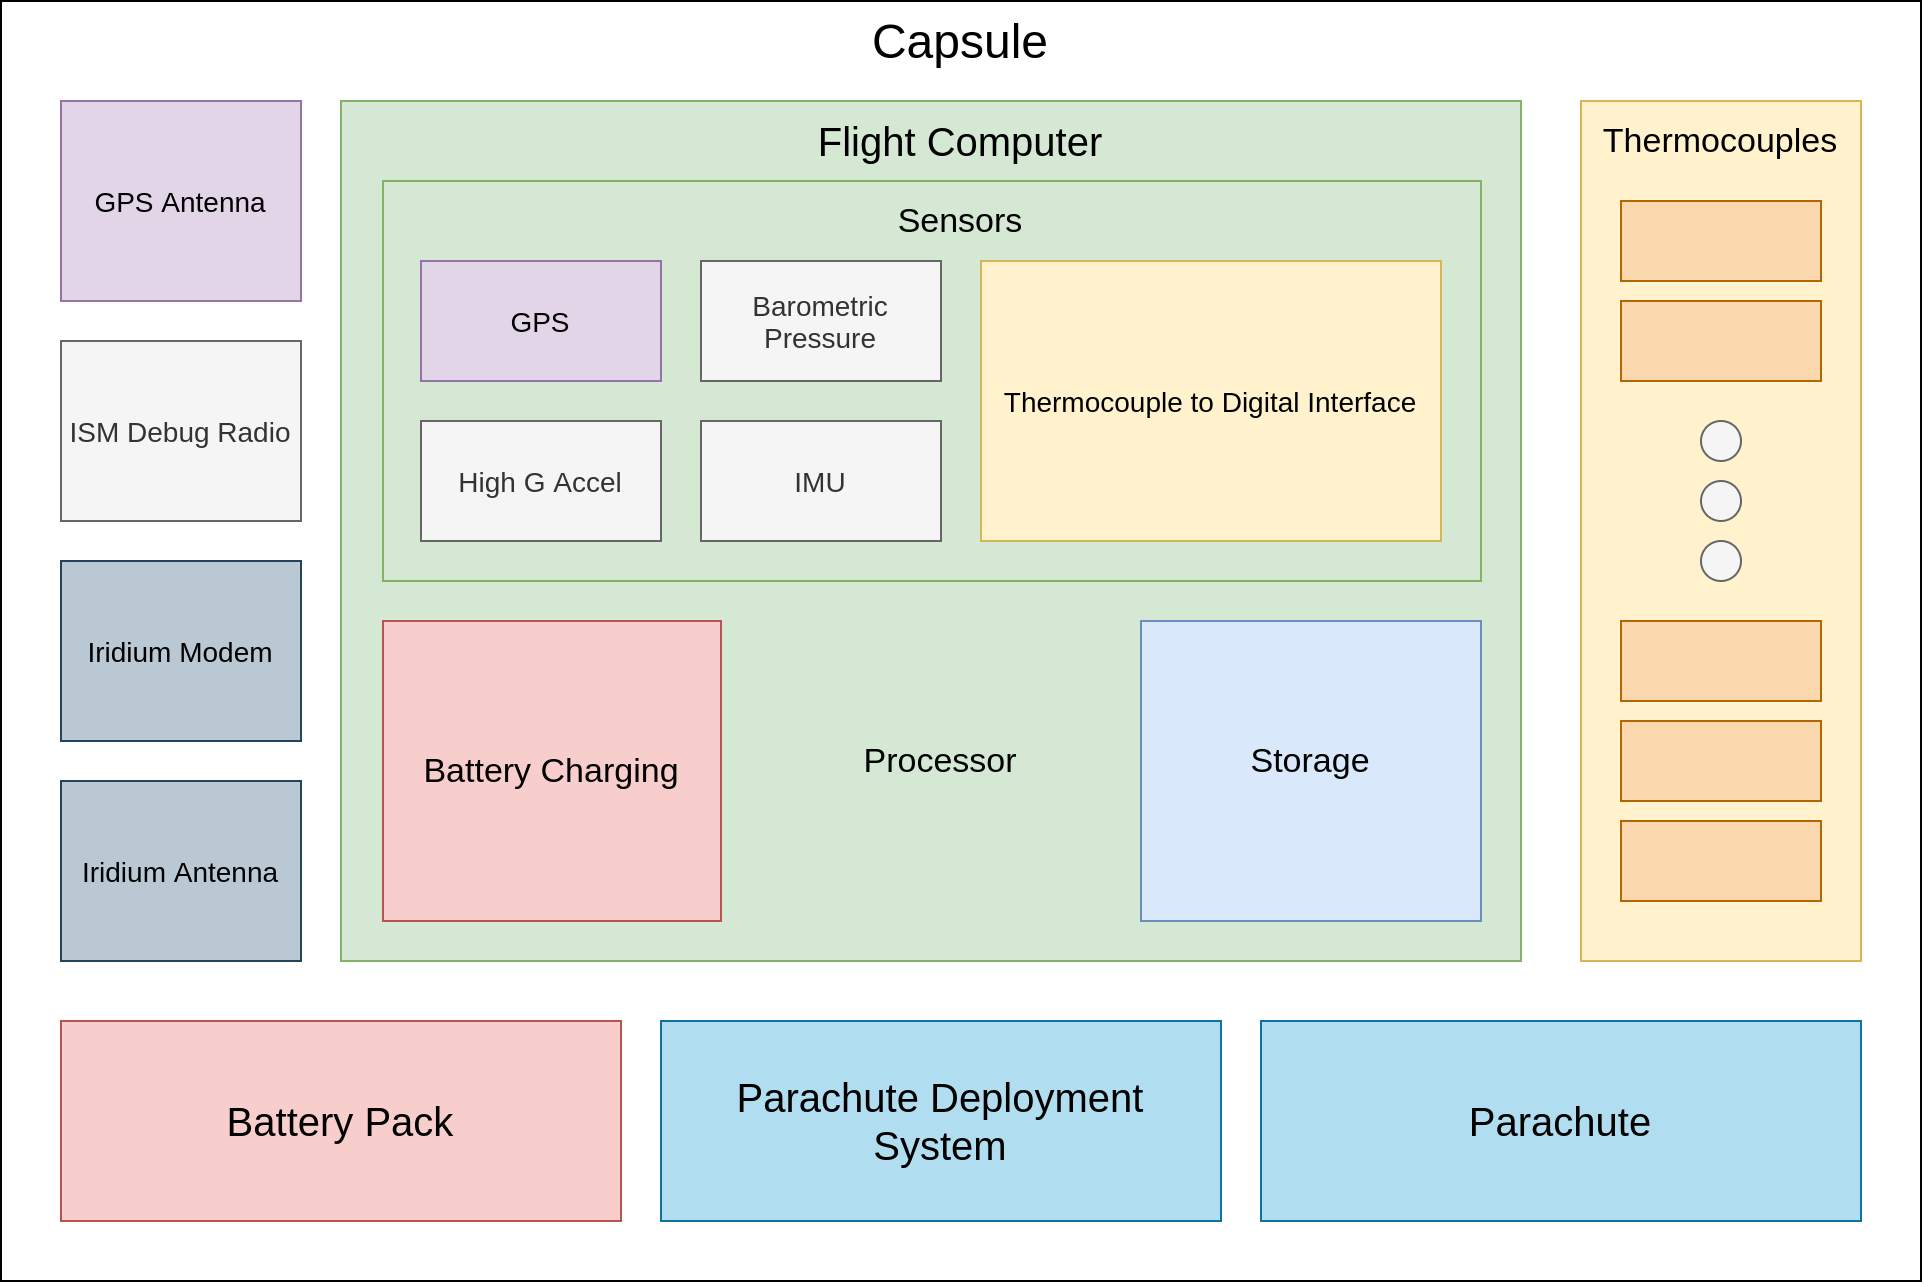
\includegraphics[width=0.95\textwidth]{images/amtps-avionics.png}
		%\caption{Capsule component overview, showing the various functional blocks.}
		%\label{fig:capsule-overview}
	\end{figure}
	
	
\end{frame}



%%%%%%%%%%%%%%%%%%%%%%%%%%%%%%%%%%%%%%%%%%%%%
%%%%%%%%%%%%%%%%%%%%%%%%%%%%%%%%%%%%%%%%%%%%%
%%%%%%%%%%%%%%%%%%%%%%%%%%%%%%%%%%%%%%%%%%%%%
\section{Temperature and Pressure Measurement}
\begin{frame}{Temperature and Pressure Measurement)}
	
	\begin{figure}[h!]
		\centering
		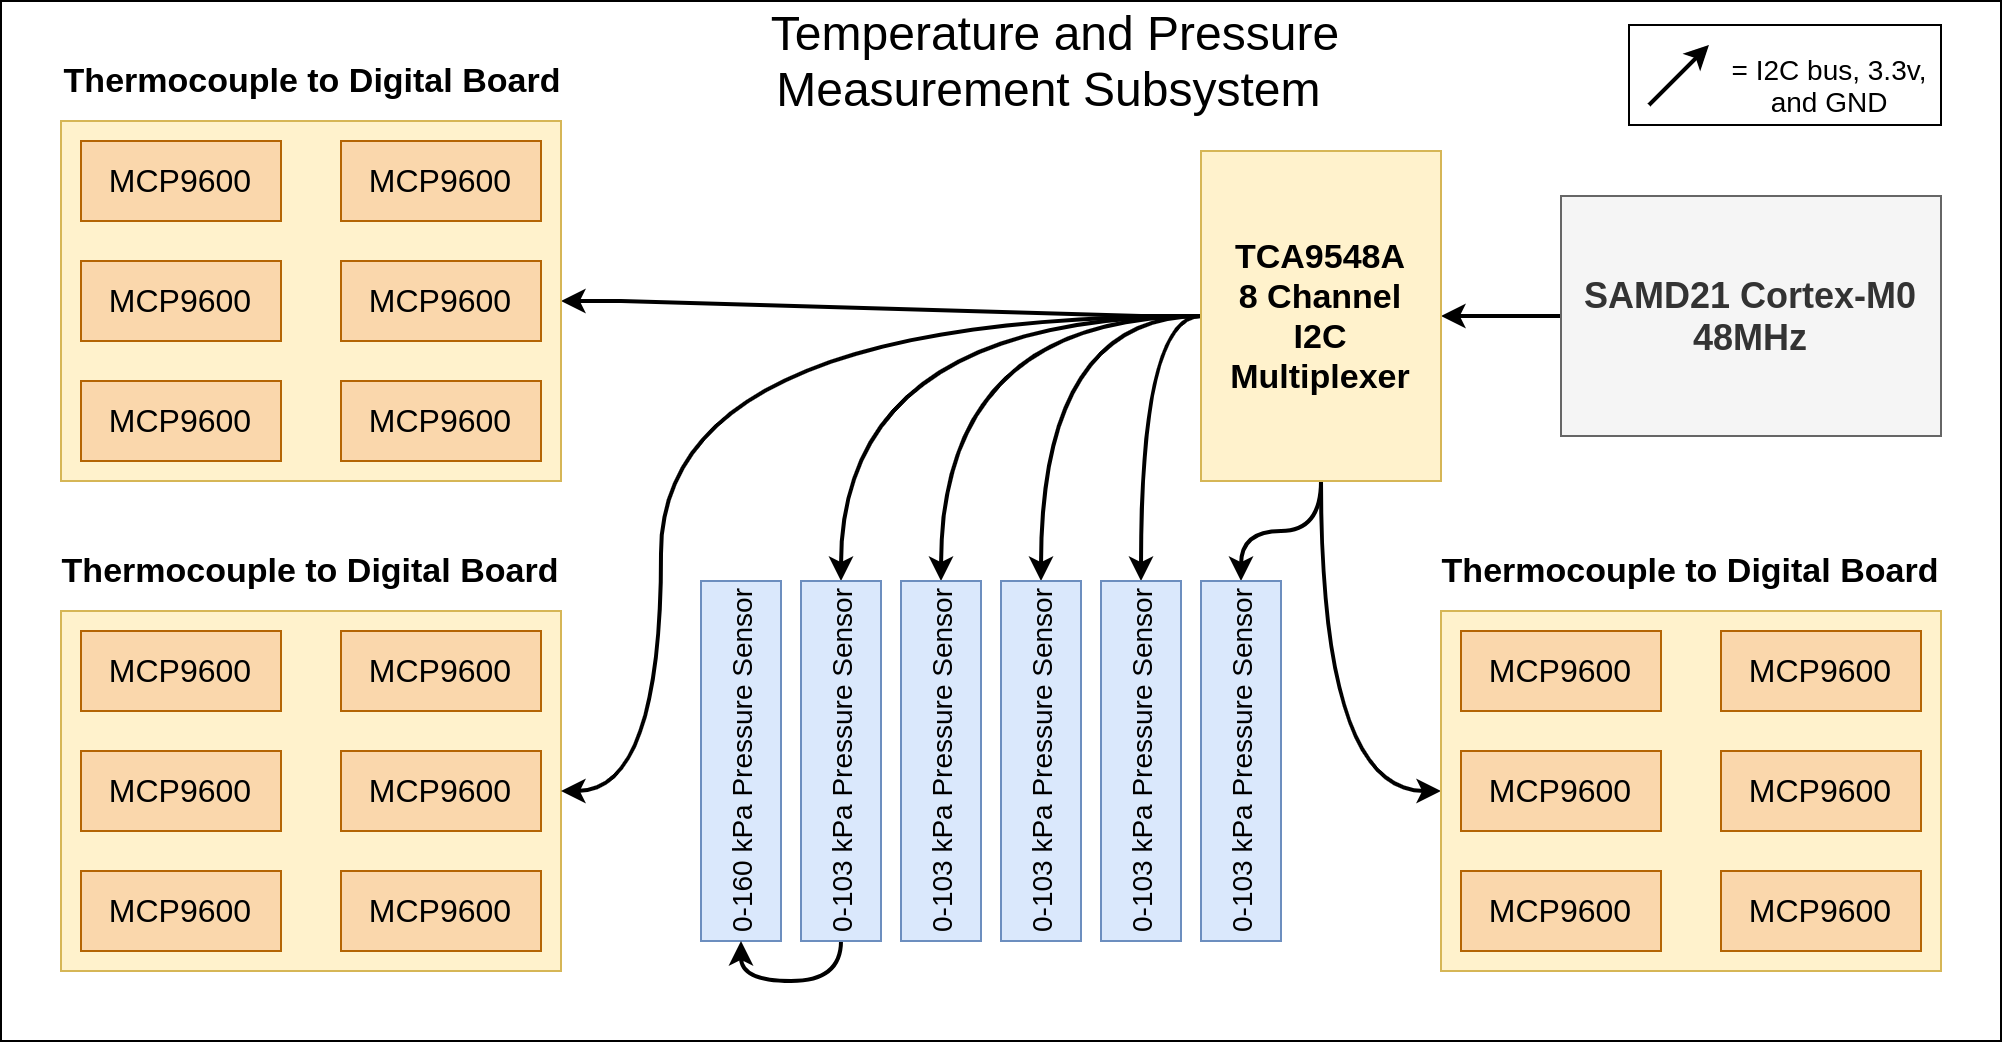
\includegraphics[width=\textwidth]{images/amtps-temp-pressure-subsystem.png}
		%\caption{Functional decomposition of the TPMS.}
		%\label{fig:tpms-overview}
	\end{figure}
	
\end{frame}


%%%%%%%%%%%%%%%%%%%%%%%%%%%%%%%%%%%%%%%%%%%%%
%%%%%%%%%%%%%%%%%%%%%%%%%%%%%%%%%%%%%%%%%%%%%
%%%%%%%%%%%%%%%%%%%%%%%%%%%%%%%%%%%%%%%%%%%%%
\section{Command and Data Handling}
\begin{frame}{Command and Data Handling}
	
	\begin{figure}[h!]
		\centering
		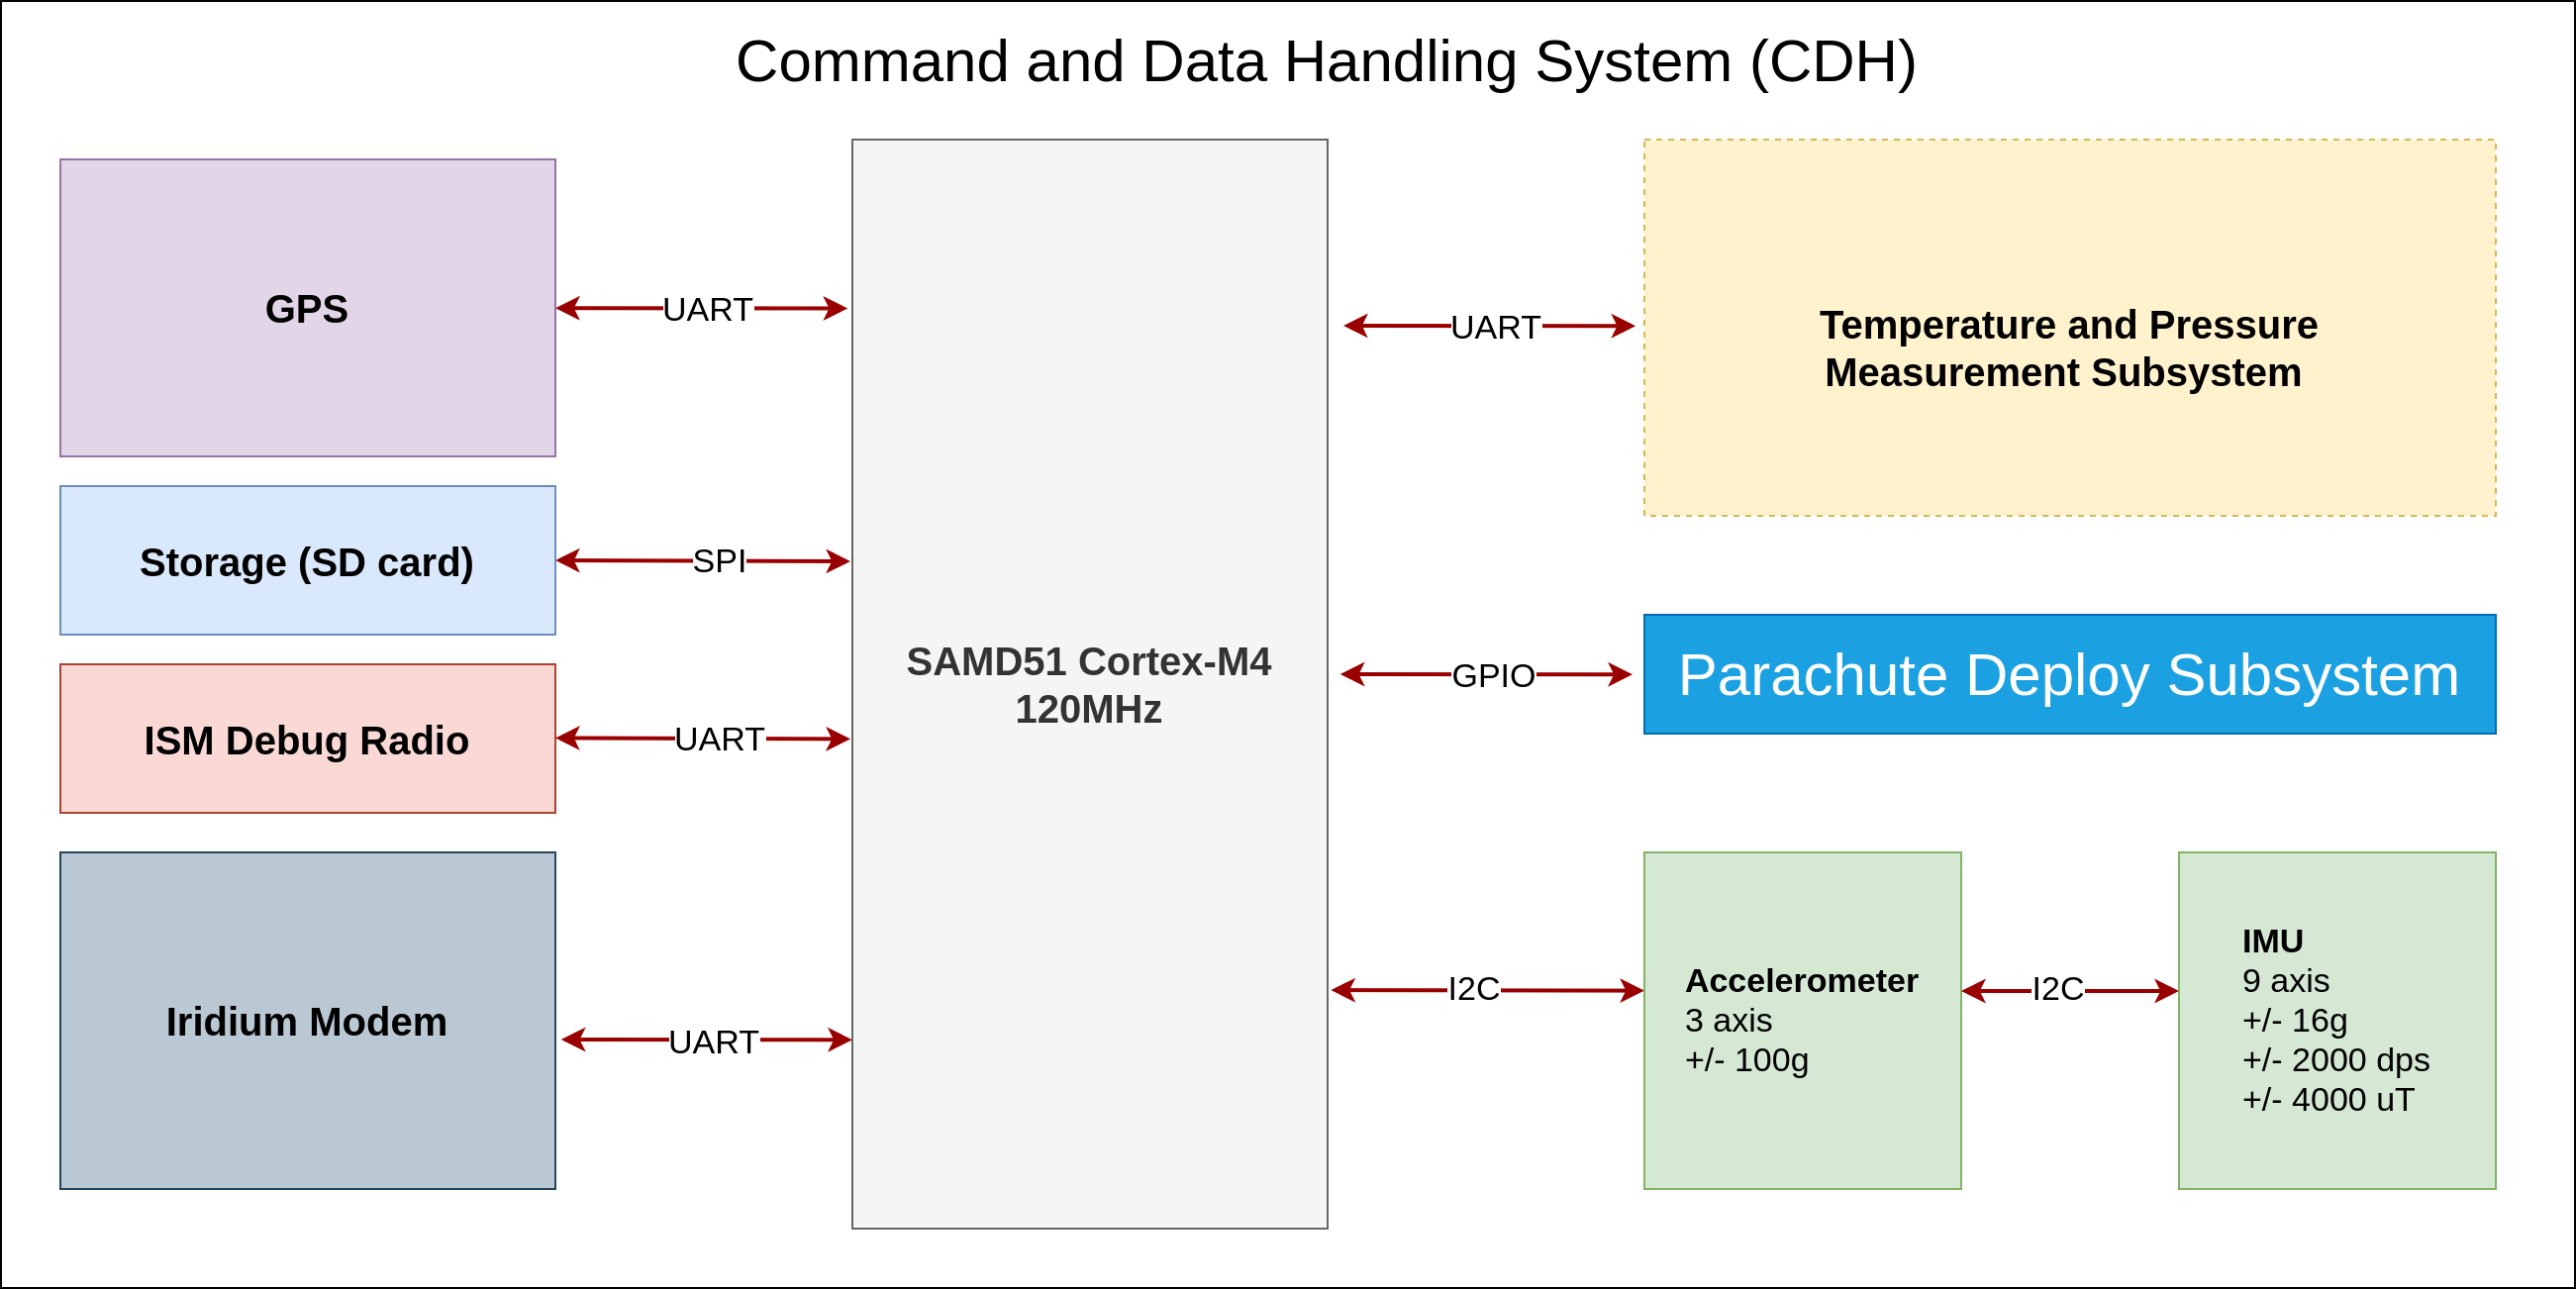
\includegraphics[width=\textwidth]{images/amtps-main-system.png}
		%\caption{Main functional components of the capsule and the communication buses between them.}
		%\label{fig:main-overview}
	\end{figure}
	
\end{frame}


%%%%%%%%%%%%%%%%%%%%%%%%%%%%%%%%%%%%%%%%%%%%%
%%%%%%%%%%%%%%%%%%%%%%%%%%%%%%%%%%%%%%%%%%%%%
%%%%%%%%%%%%%%%%%%%%%%%%%%%%%%%%%%%%%%%%%%%%%
\section{Software Design}
\begin{frame}{Parachute Control}

	\begin{figure}[h!]
		\centering
		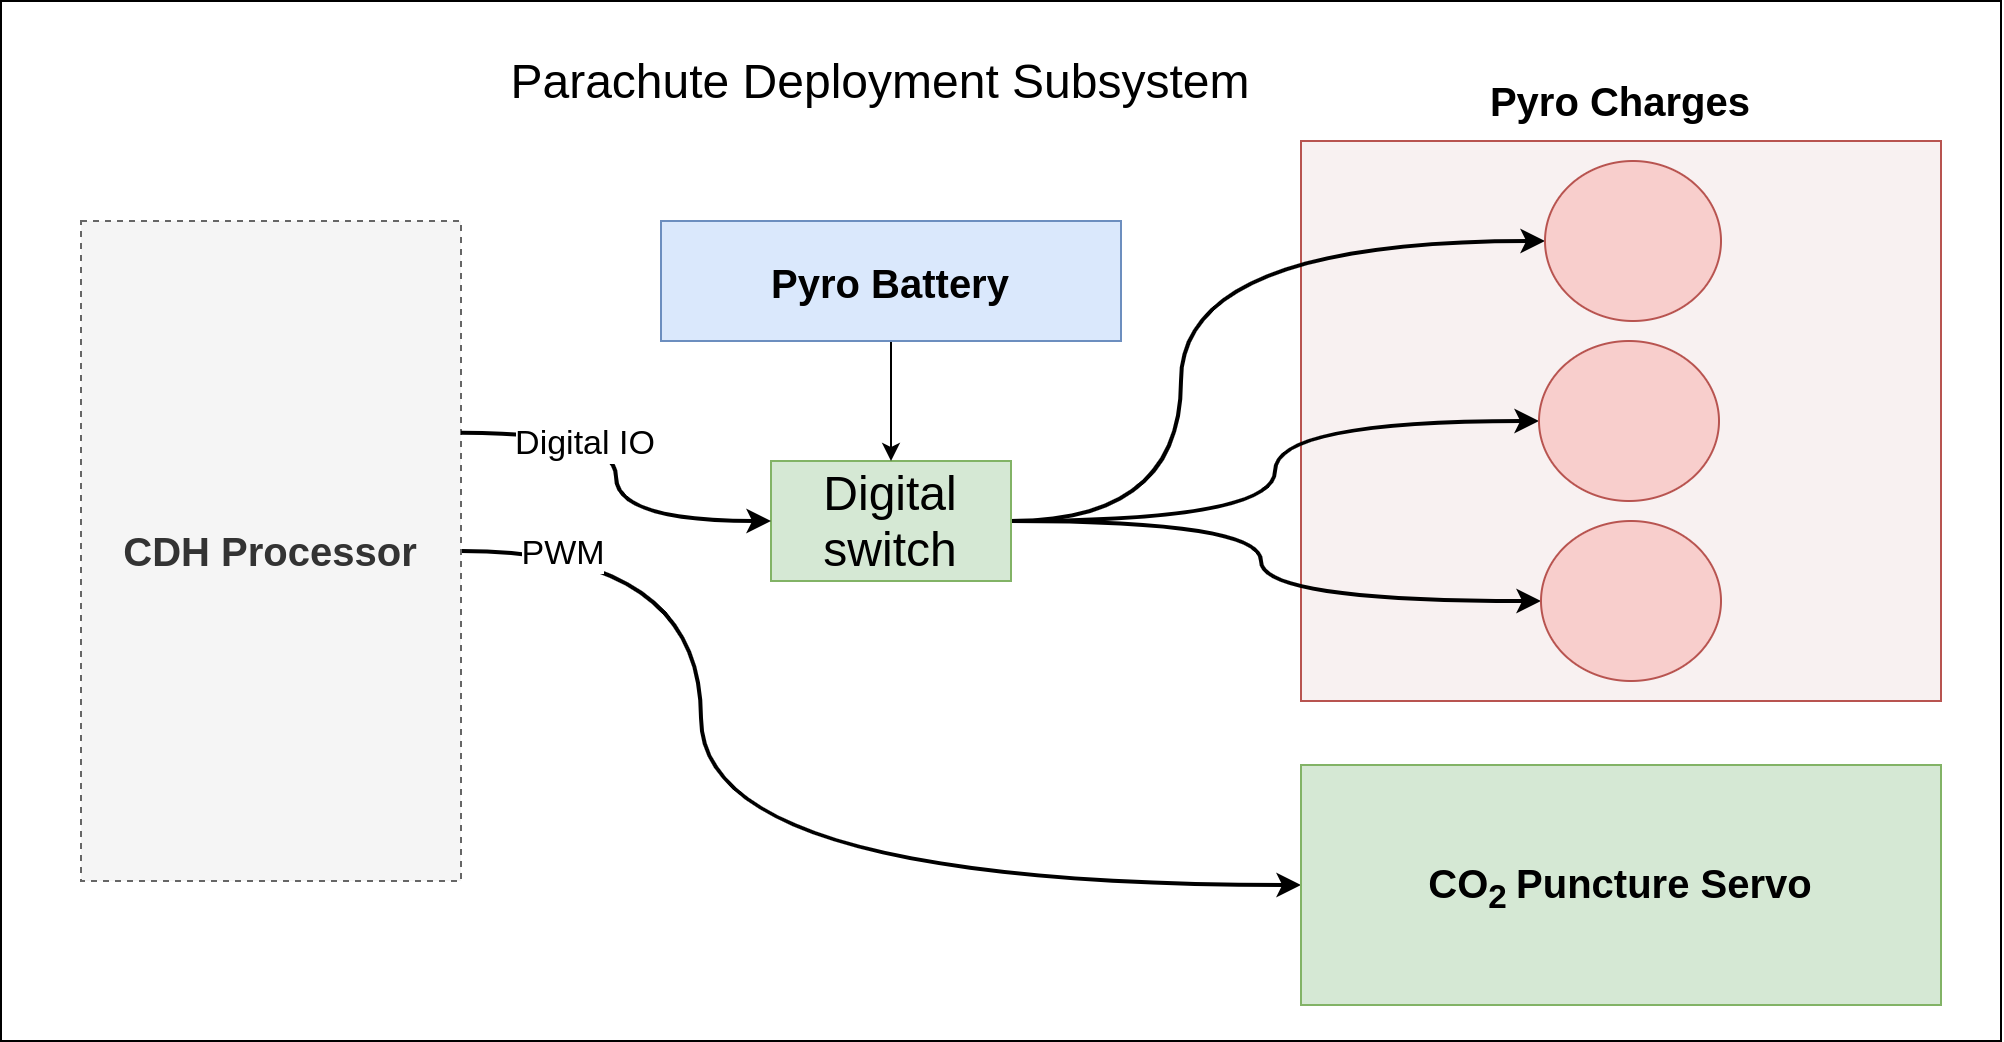
\includegraphics[width=\textwidth]{images/amtps-parachute.png}
		%\caption{Main functional components of the capsule and the communication buses between them.}
		%\label{fig:main-overview}
	\end{figure}
	
\end{frame}


%%%%%%%%%%%%%%%%%%%%%%%%%%%%%%%%%%%%%%%%%%%%%
%%%%%%%%%%%%%%%%%%%%%%%%%%%%%%%%%%%%%%%%%%%%%
%%%%%%%%%%%%%%%%%%%%%%%%%%%%%%%%%%%%%%%%%%%%%
\section{Prototype Hardware}
\begin{frame}[allowframebreaks]{Prototype Hardware}
	
	\begin{figure}[h!]
		\centering
		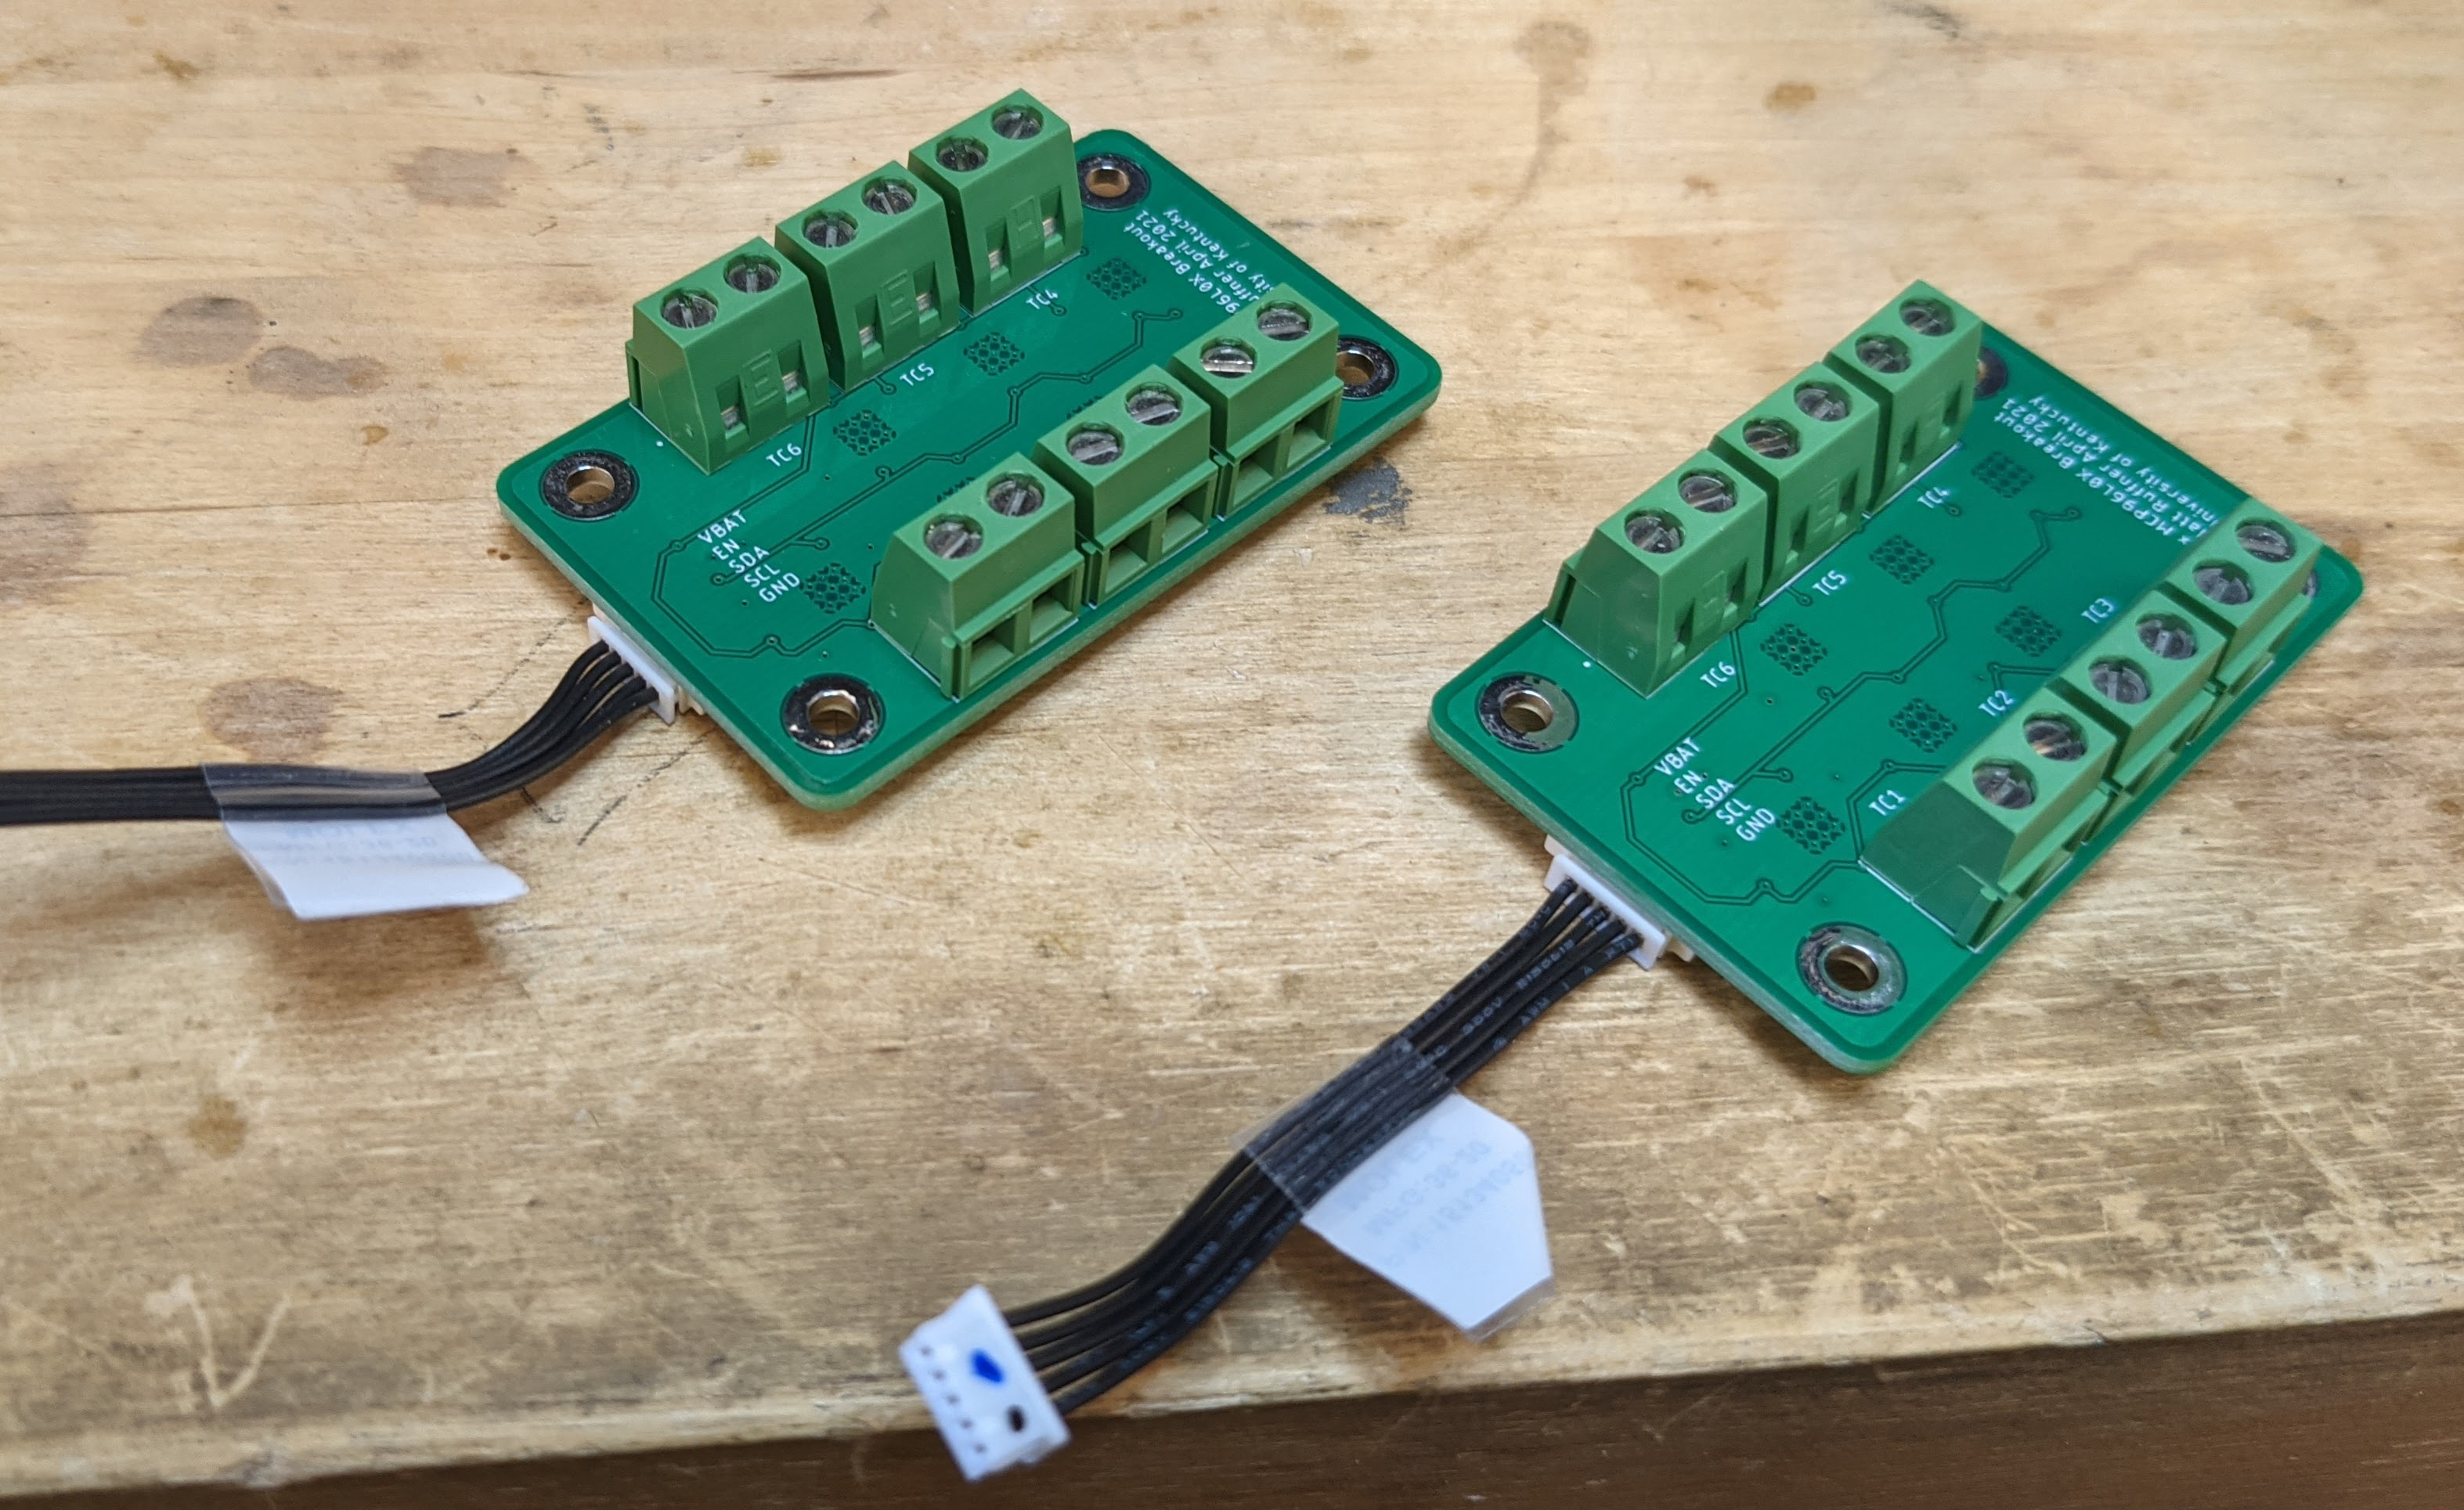
\includegraphics[width=0.8\textwidth]{images/tc-board-top.jpg}
		\caption{Six channel MCP9600 breakout (top).}
		%\label{fig:tpms-overview}
	\end{figure}
	
	\begin{figure}[h!]
		\centering
		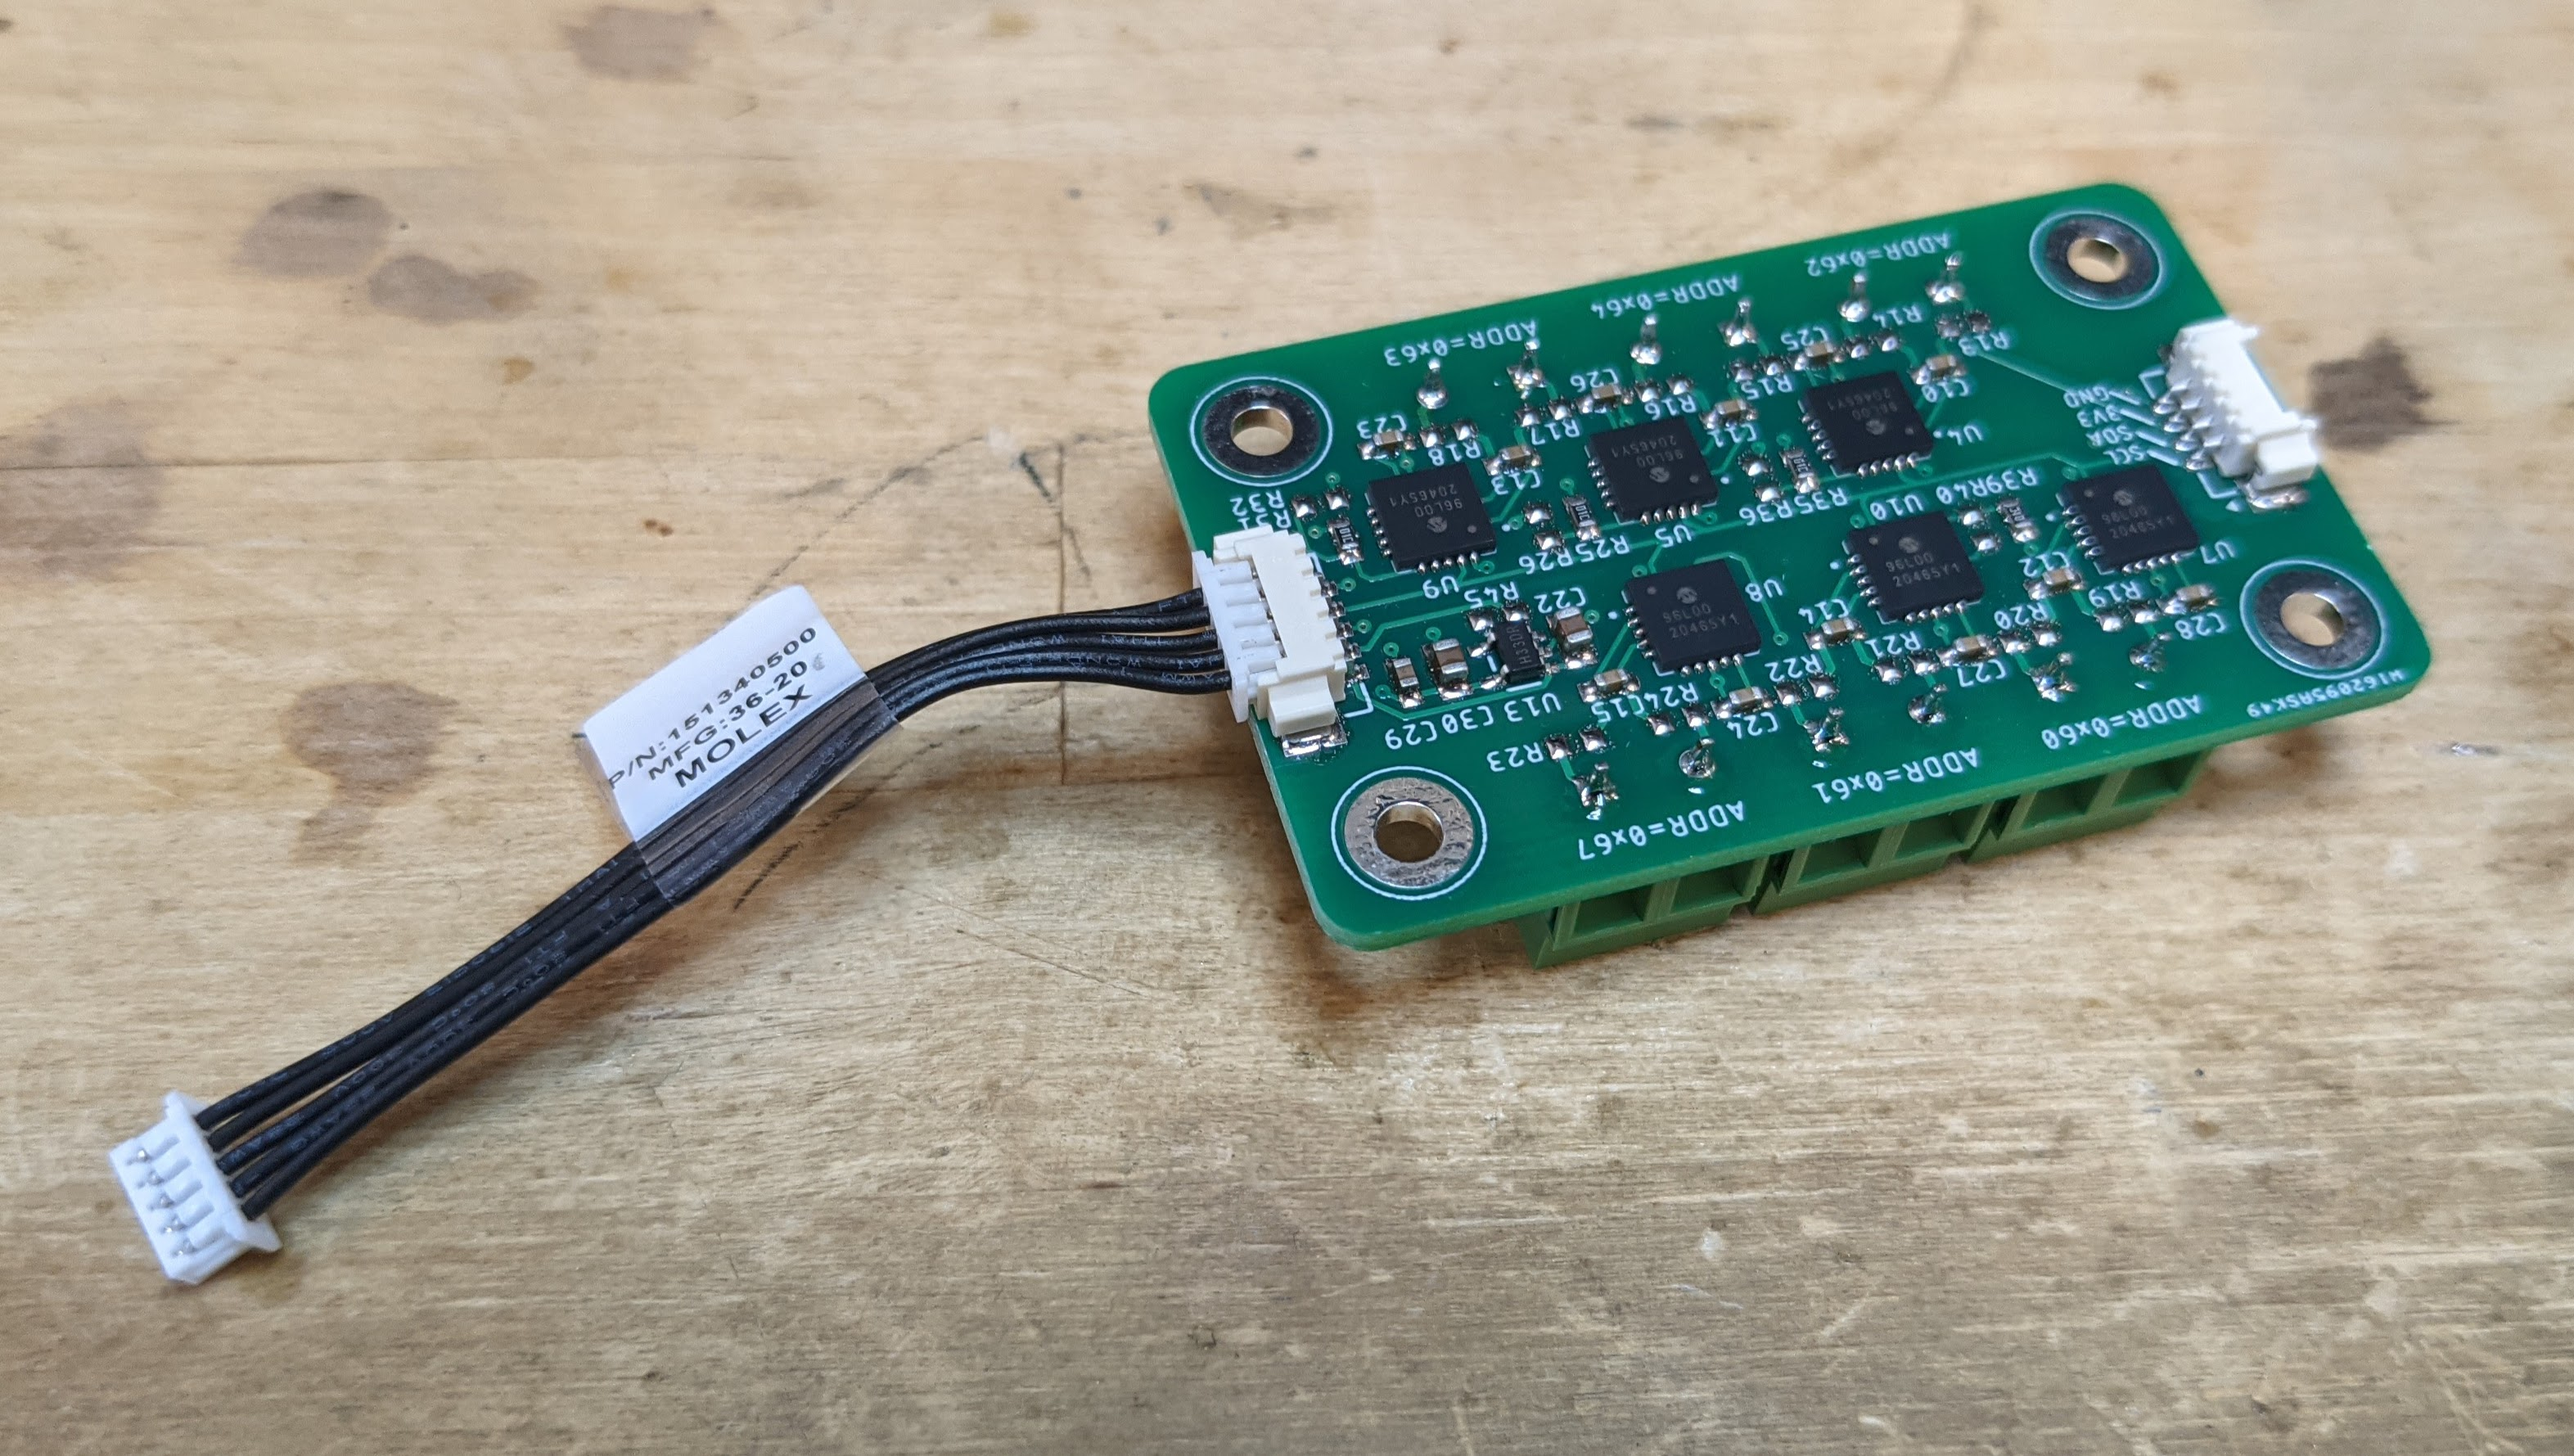
\includegraphics[width=0.8\textwidth]{images/tc-board-bottom.jpg}
		\caption{Six channel MCP9600 breakout (bottom).}
		%\label{fig:tpms-overview}
	\end{figure}
	
	\begin{figure}[h!]
		\centering
		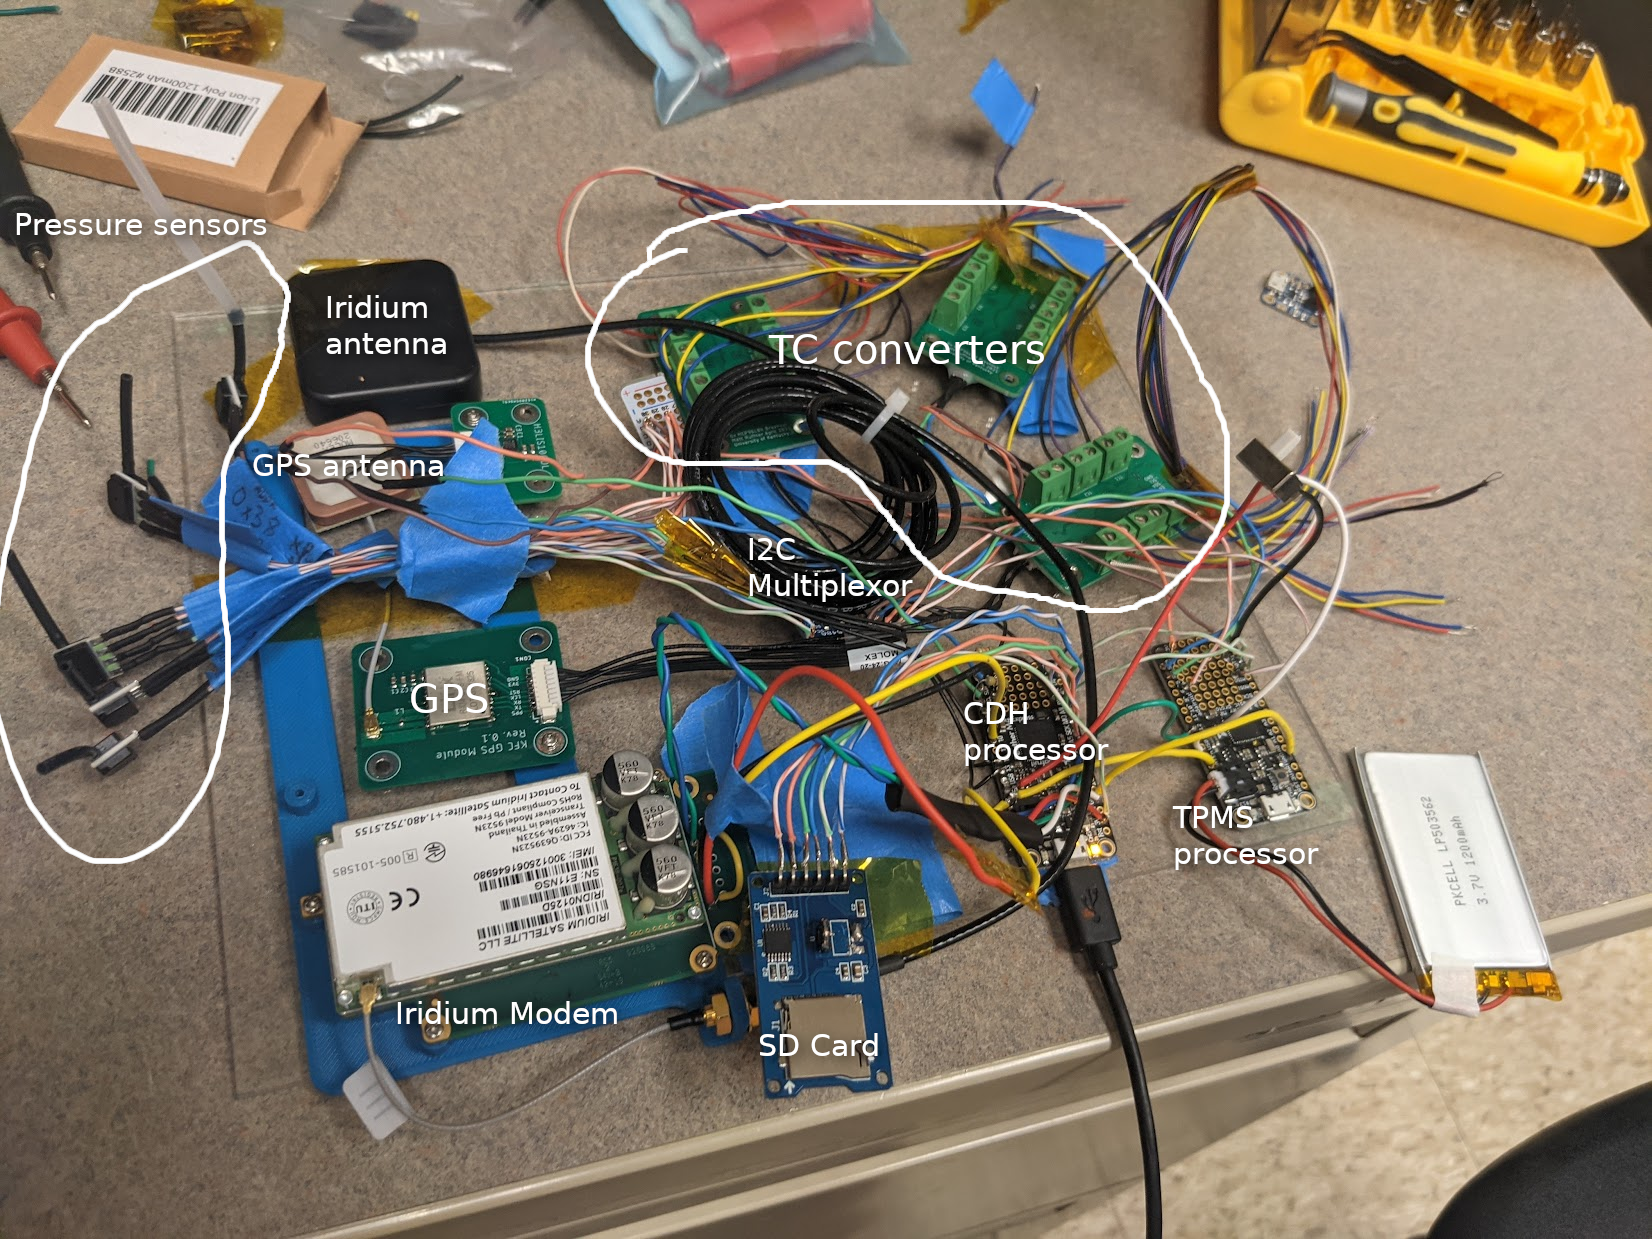
\includegraphics[width=0.9\textwidth]{images/subsystem-hardware-annotated.png}
		\caption{Full system.}
		%\label{fig:tpms-overview}
	\end{figure}

	
\end{frame}


\section{Final Design Considerations}
\begin{frame}[allowframebreaks]{Final Design Considerations}
	
	\begin{itemize}
		\item \textbf{Supply chain constraints} - bare SAMD21/51 processors are hard to find on Digikey/Mouser etc. but pre-made development boards from Adafruit are still available.
	\end{itemize}	

	\begin{figure}[h!]
		\begin{subfigure}{0.4\textwidth}
			\centering
			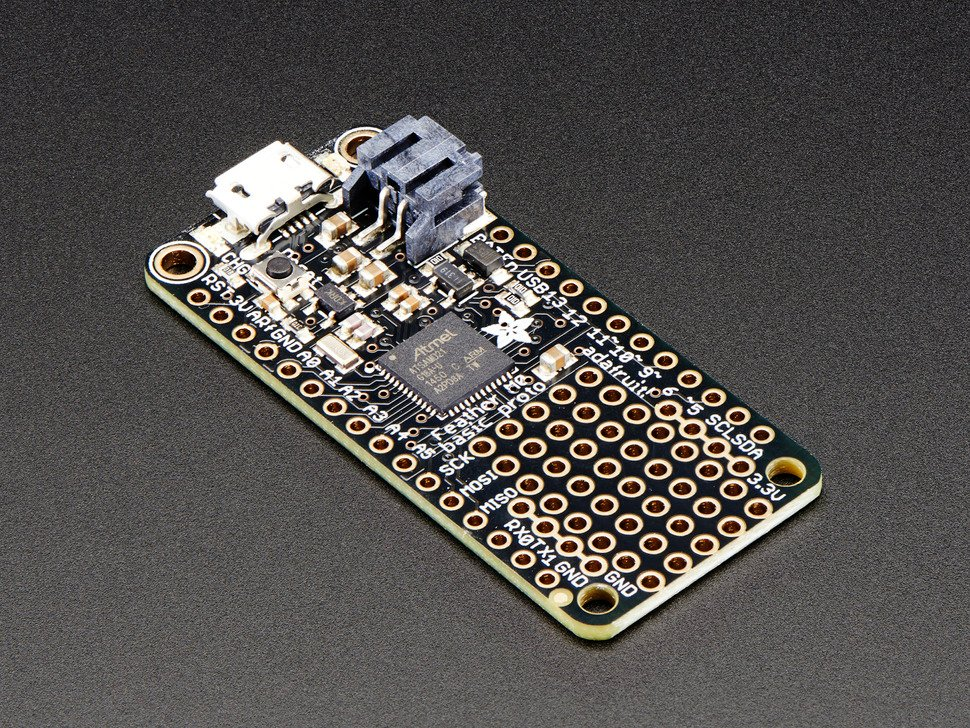
\includegraphics[width=\textwidth]{images/featherm0.jpg}
			\caption{Adafruit SAMD21 48MHz Cortex-M0 carrier \tiny{\url{https://www.adafruit.com/product/2772}}}
		\end{subfigure}
		\qquad
		\begin{subfigure}{0.4\textwidth}
			\centering
			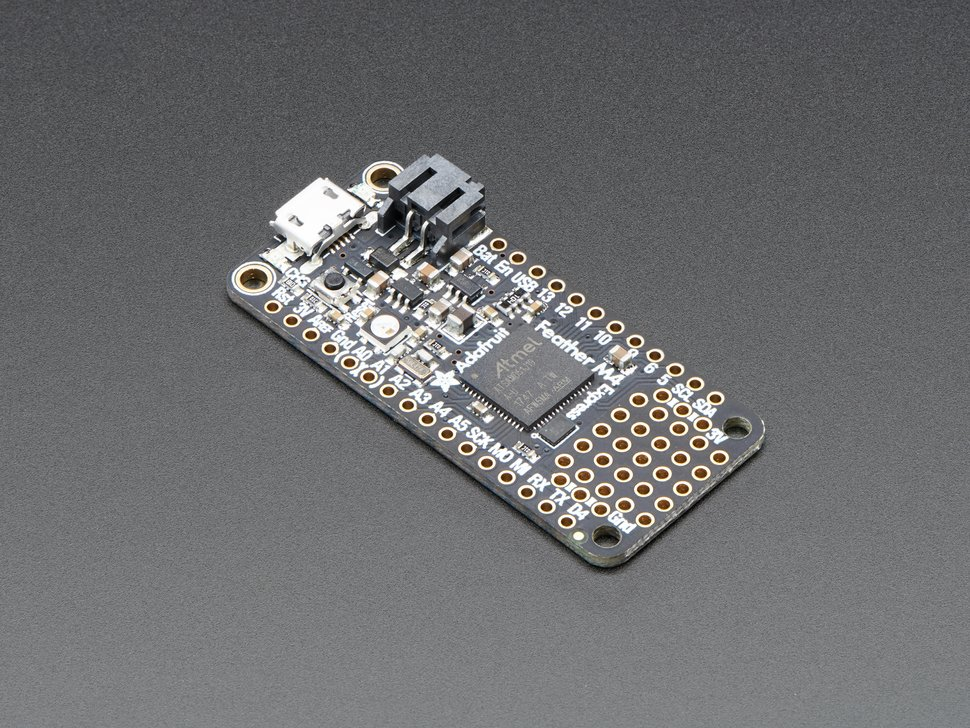
\includegraphics[width=\textwidth]{images/featherm4.jpg}
			\caption{Adafruit SAMD51 120MHz Cortex-M4 carrier \tiny{\url{https://www.adafruit.com/product/3857}}}
		\end{subfigure}
		%\label{fig:tpms-overview}
	\end{figure}

	\begin{itemize}
		\item \textbf{Plenty of processor overhead} - recording 12 channels of IMU and accelerometer data to an SD card at 100Hz requires strict timing and interrupt handling
		\item Current planned revision is to separate IMU and high-g accelerometer interfacing to its own Cortex-M0 processor.
	\end{itemize}

	\begin{figure}
		\centering
		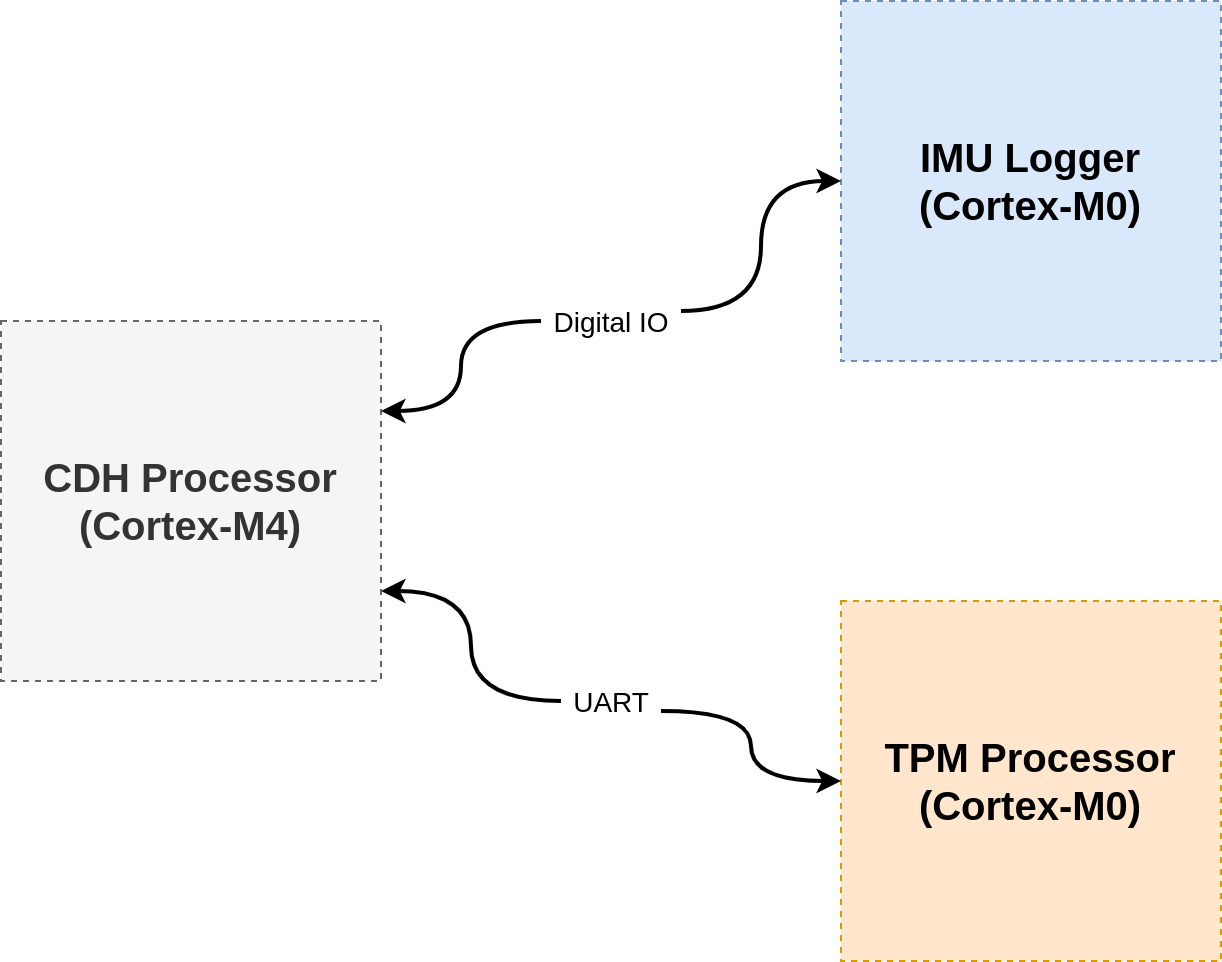
\includegraphics[width=0.4\textwidth]{images/amtps-processor-setup.png}
		\caption{Processor separation of responsibilities.}		
	\end{figure}

\end{frame}

\section{Final PCB Designs}
\begin{frame}[allowframebreaks]{Rev 2 board designs}
	
	\begin{figure}[h!]
		\centering
		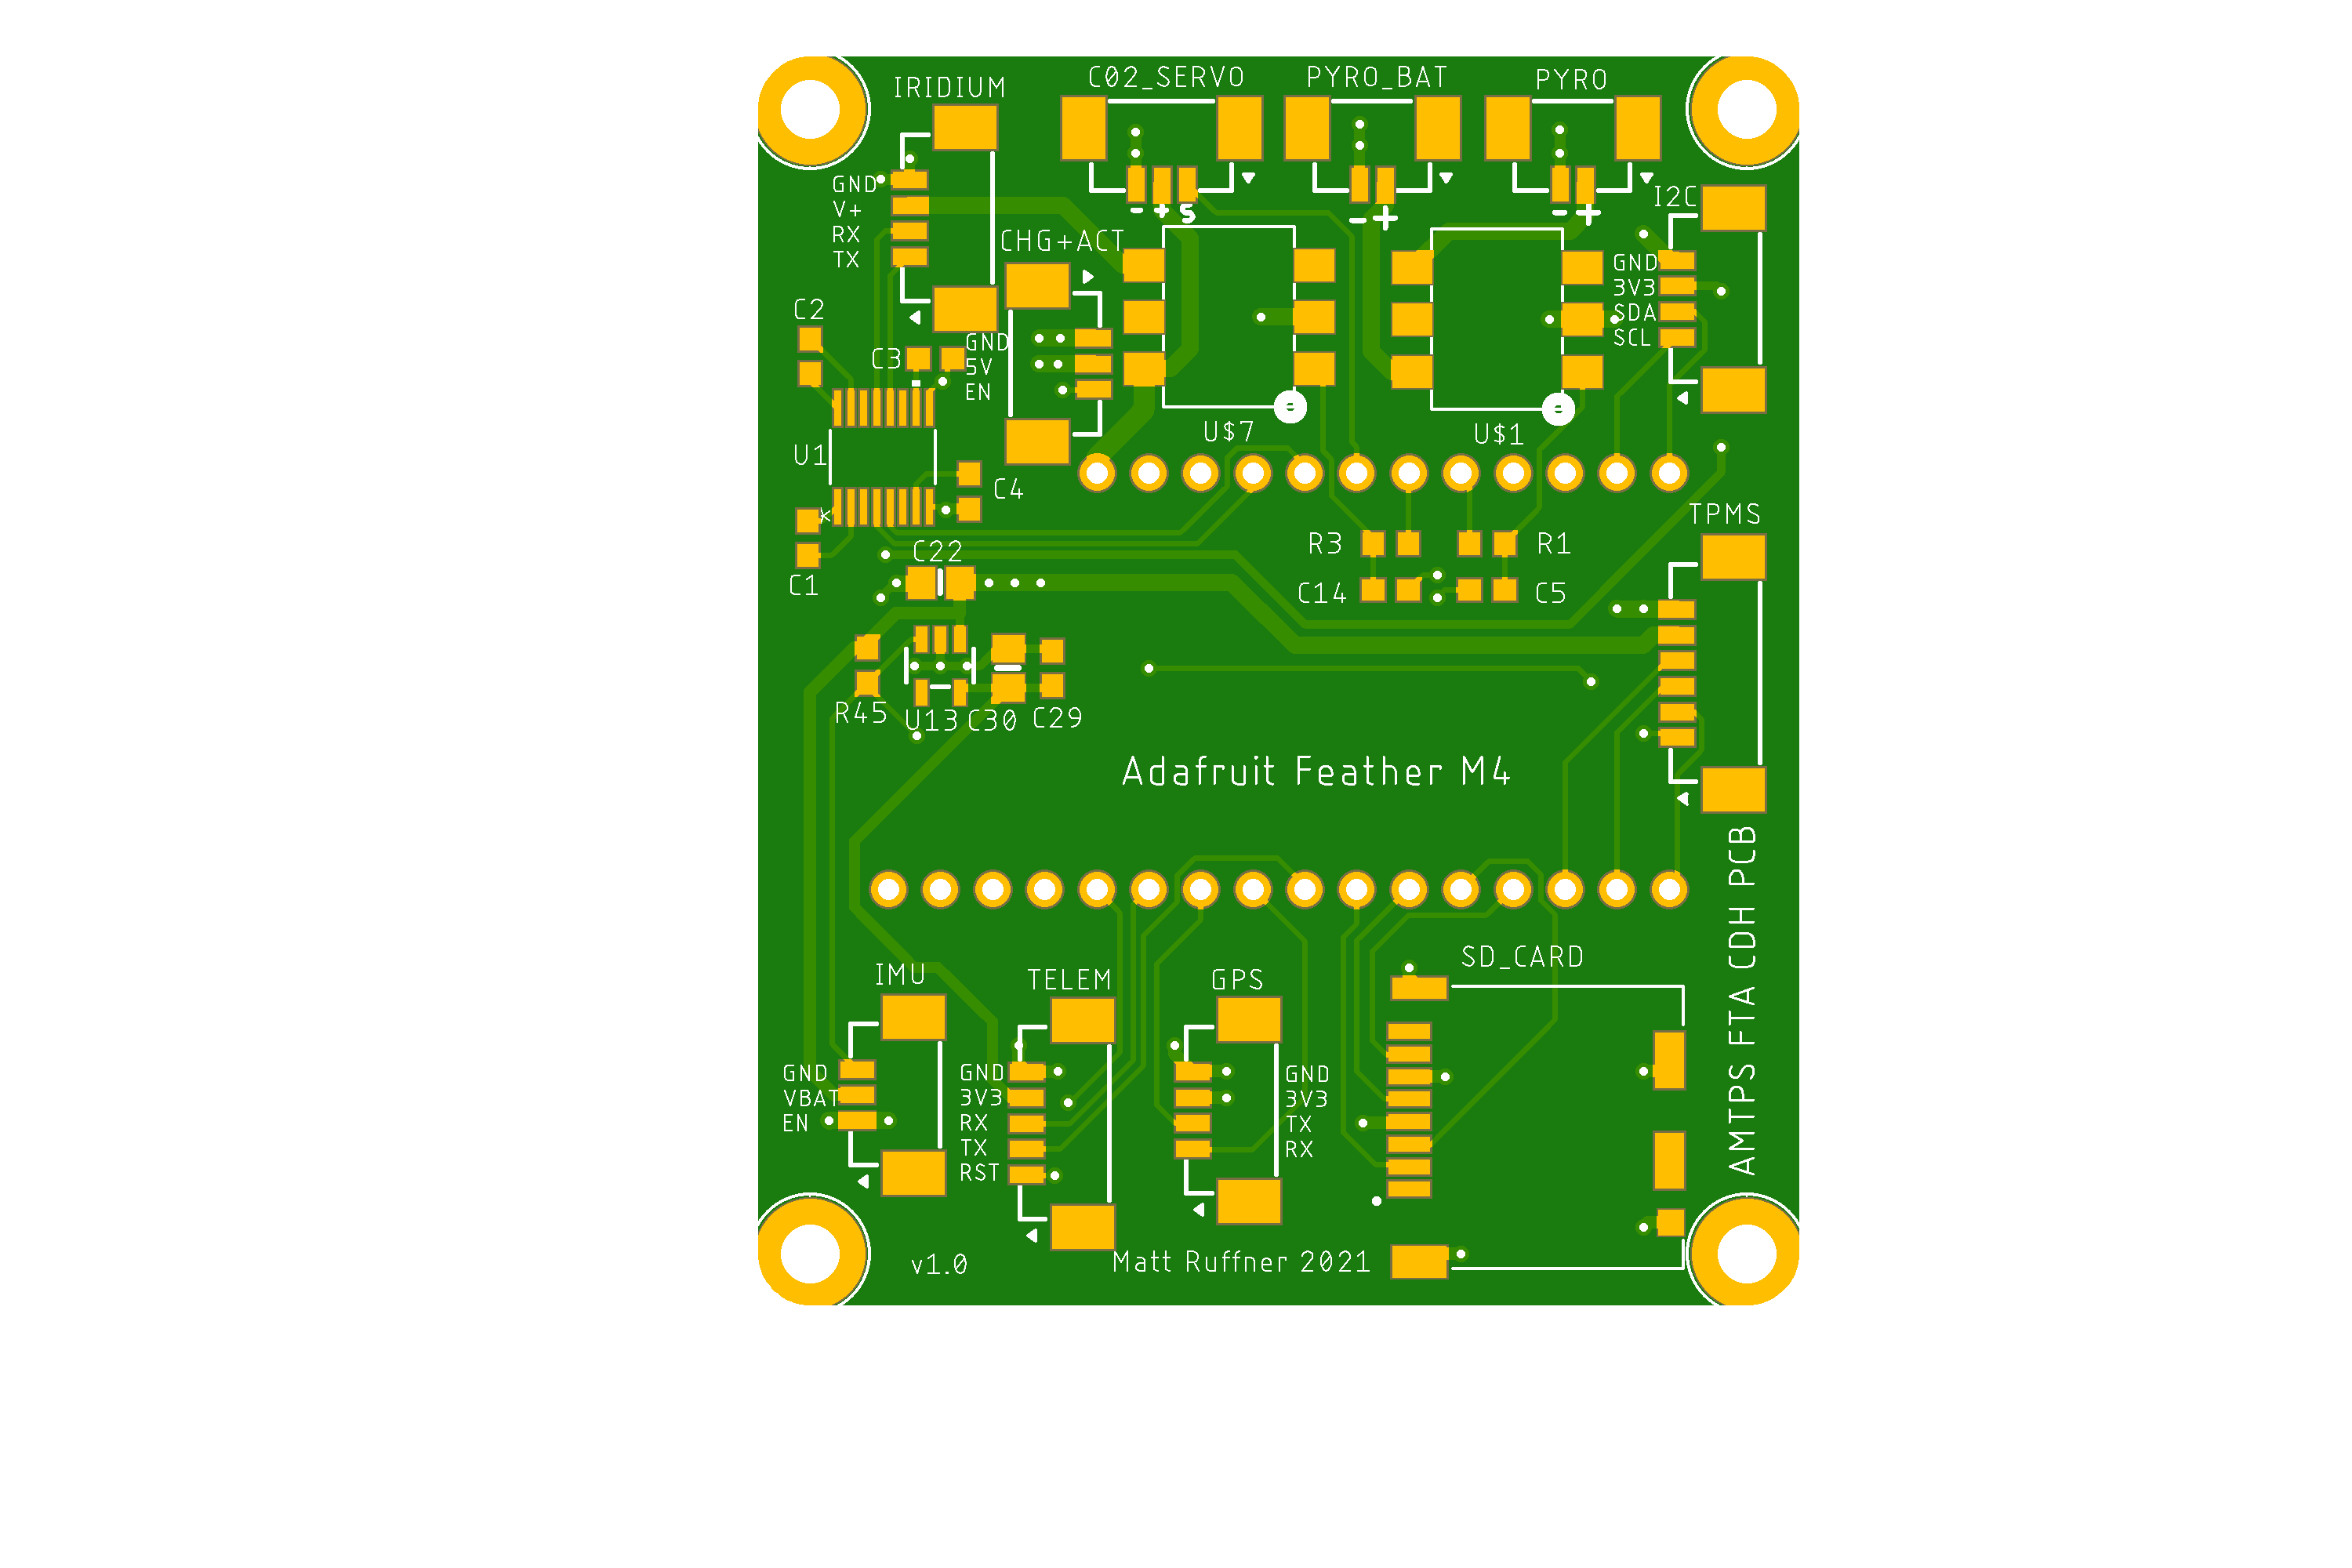
\includegraphics[width=0.8\textwidth]{images/main_board.png}
		\caption{CDH processor carrier PCB.}
		%\label{fig:tpms-overview}
	\end{figure}

	\begin{figure}[h!]
		\centering
		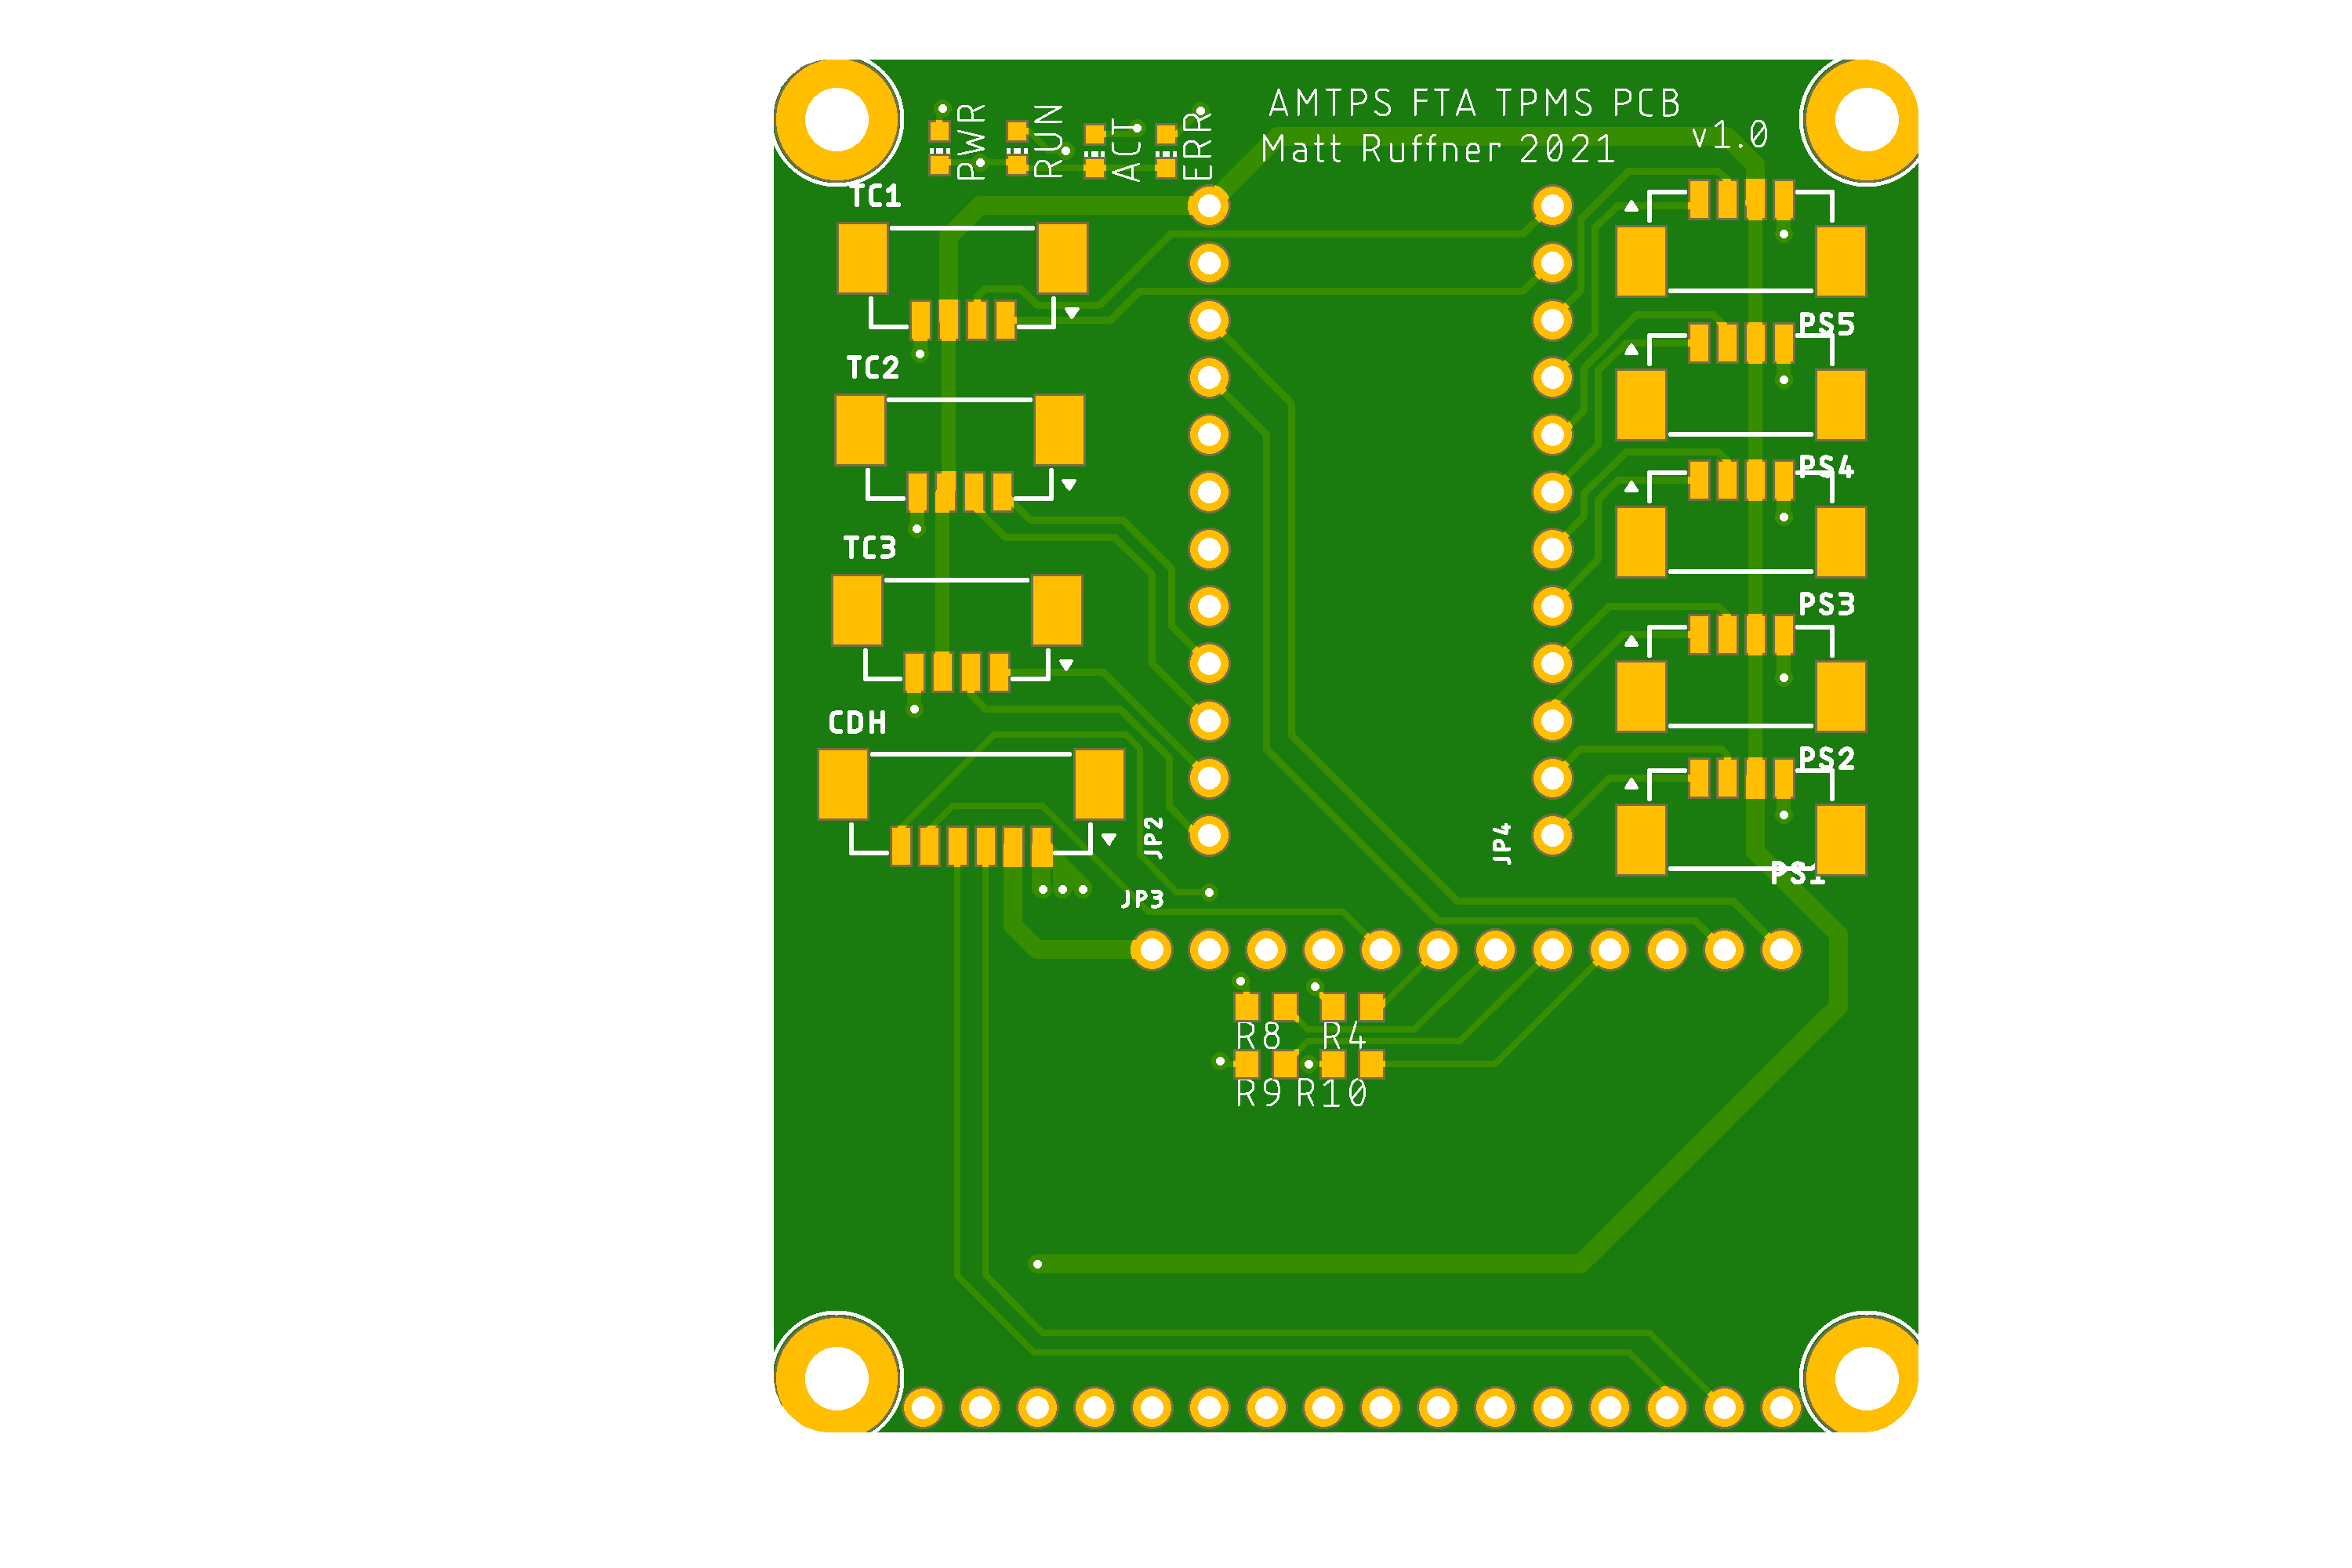
\includegraphics[width=0.8\textwidth]{images/tpms_breakout.png}
		\caption{TMP processor carrier PCB.}
		%\label{fig:tpms-overview}
	\end{figure}

	\begin{figure}[h!]
		\centering
		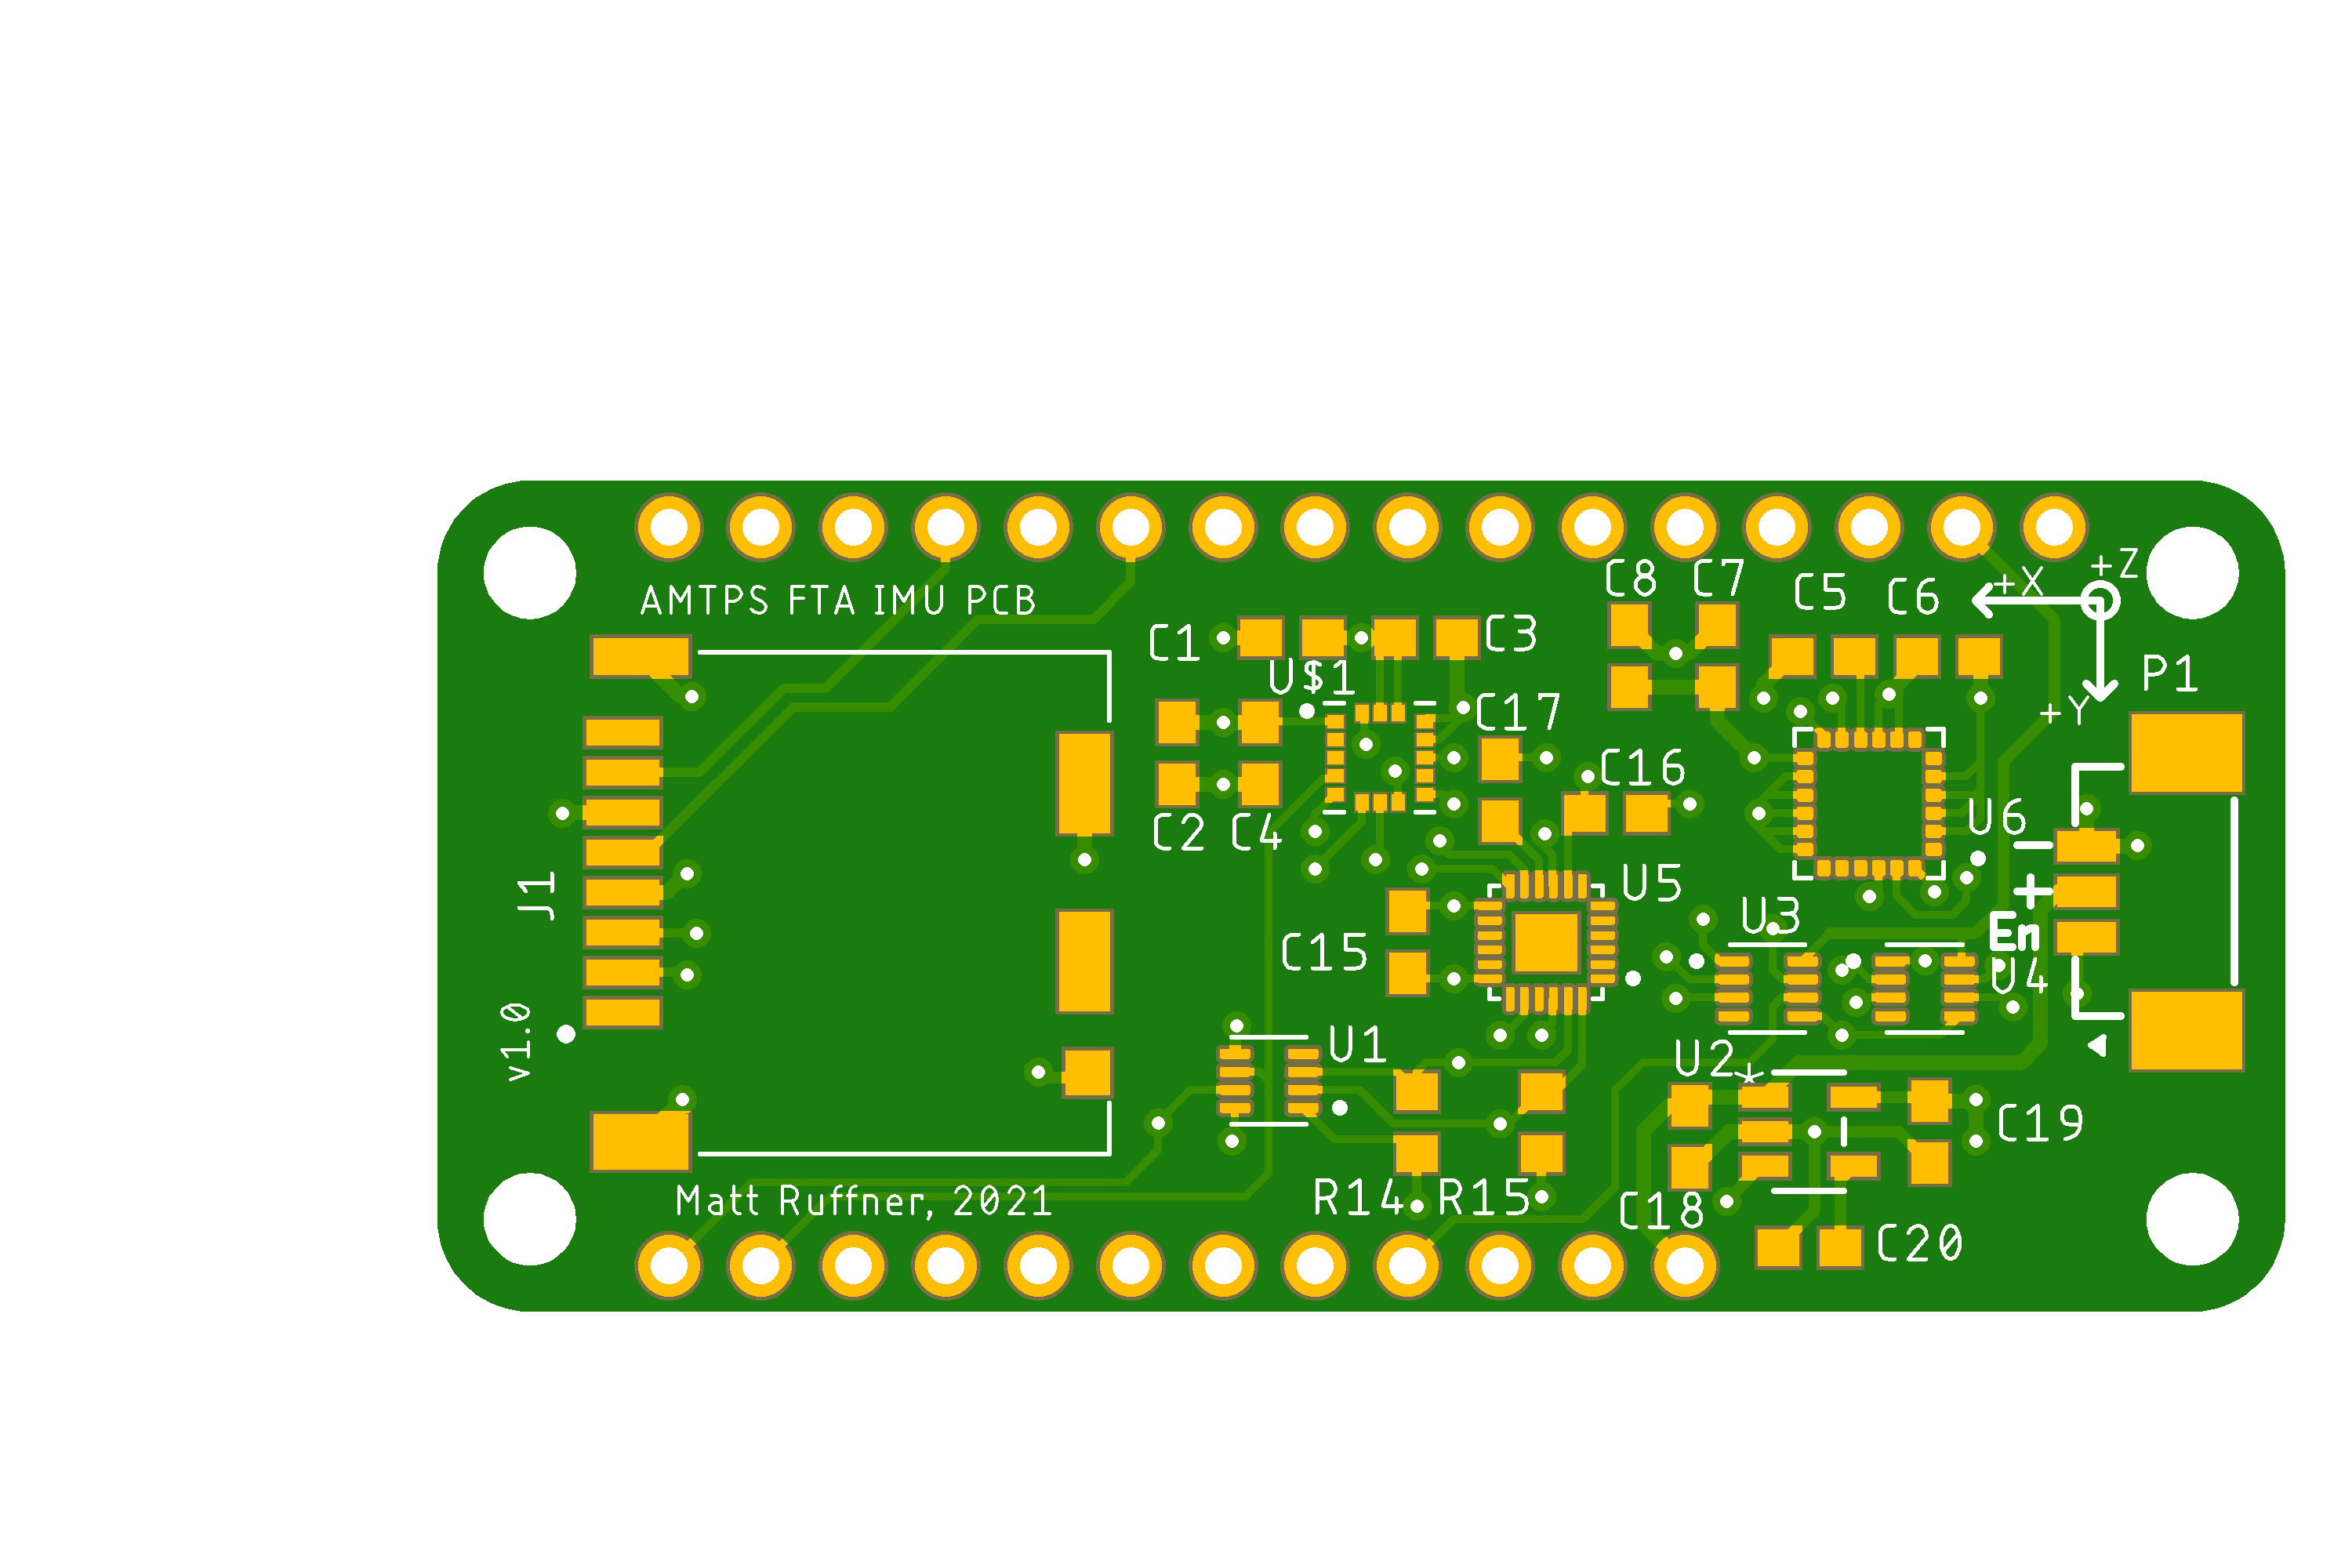
\includegraphics[width=0.8\textwidth]{images/imu_logger.png}
		\caption{IMU logger processor carrier PCB.}
		%\label{fig:tpms-overview}
	\end{figure}

\end{frame}

\section{Software Design}
\begin{frame}{Software Overview}
	
	\begin{itemize}
		\item Adafruit Feather line of boards is Arduino compatible
		\item SAMD21/51 series of processors has easily reconfigurable SERCOMs to support multiple hardware serial ports 
		\item FreeRTOS Queues and Semaphores allow for simple and reliable transfer of data and atomic hardware access
		\item Open source libraries available for all sensors
		\item All hardware design files and firmware, as well as ground assist tools for plotting recorded data are version controlled on private Github repositories:
		\begin{itemize}
			\item \url{https://github.com/krups/amtps-fta-hardware}
			\item \url{https://github.com/krups/amtps-fta-software}
		\end{itemize}	
	\end{itemize}
	
\end{frame}




\end{document}
